%\documentclass[a4paper,12pt]{report}
%\documentclass[letter,12pt]{report}
 \documentclass[a4paper,12pt]{book}


\usepackage[utf8]{inputenc}
\usepackage[spanish]{babel}\decimalpoint
\usepackage{babel}
\selectlanguage{spanish}
%\usepackage{pdftricks}
%\usepackage{epstopdf}
%\usepackage{pst-pdf}
% \usepackage{purifyeps}
% \usepackage{pstoedit}
% \usepackage{color}
\usepackage{graphics}
\usepackage{graphicx}
\usepackage{tocbibind}
\RequirePackage[colorlinks=false,hyperindex]{hyperref}
\usepackage{psfrag}
\usepackage{pstricks}
\usepackage{xcolor}
%\usepackage{pst-grad}
%\usepackage{pst-3d}
%\usepackage{pst-3dplot}
%\usepackage{pst-fr3d}
%\usepackage{pst-gr3d}
%\usepackage{pst-map3dII}
%\usepackage{pst-vue3d}
%\usepackage{fancybox}
%\usepackage{pst-node}
%\usepackage{pst-tree}
%\usepackage[fixlanguage]{babelbib}
\usepackage{setspace} 
%\usepackage{float}
\usepackage{amsmath,amsfonts,amssymb}
%\usepackage{appendix}
% \usepackage{chapterbib}
%\usepackage{draftcopy}

%\usepackage{type1cm,eso-pic,color}

% \makeatletter
% \AddToShipoutPicture{%
% \setlength{\@tempdimb}{.5\paperwidth}%
% \setlength{\@tempdimc}{.5\paperheight}%
% \setlength{\unitlength}{1pt}%
% \put(\strip@pt\@tempdimb,\strip@pt\@tempdimc){%
% \makebox(0,0){\rotatebox{45}{\textcolor[gray]{0.95}%
% {\fontsize{3cm}{3cm}\selectfont{PRELIMINAR}}}}%
% \makebox(-100,-300){\rotatebox{45}{\textcolor[gray]{0.95}%
% {\fontsize{2cm}{2cm}\selectfont{USO EXCLUSIVO DEL \\ CONICET}}}}
% \makebox(-500,-0){\rotatebox{90}{\textcolor[gray]{0.95}%
% {\fontsize{0.7cm}{0.7cm}\selectfont{\textcopyright Copyright 2011 - Demian Slobinsky}}}}
% }%
% }
% \makeatother


\usepackage{fancyhdr}
\pagestyle{fancy}
\fancyhead[ER]{}
\fancyhead[OL]{}
%\fancyfoot[LO,RE]{\thepage
\newcommand{\figwidth}{0.9\columnwidth}
\newcommand{\mean}[1]{\ensuremath{\langle #1 \rangle}}
\newcommand{\abs}[1]{\left\vert#1\right\vert}

%% reset figure counters at the beginning of each chapter
%\newcommand{\Section}[1]{\section{#1} \setcounter{figure}{1}}

\renewcommand{\thefigure}{\arabic{figure}}

% con esto evito que me muestre los numeros de chapter
% ya que mi "book" tiene un solo chapter, sino me numeraria
% todo 1.algo
\renewcommand*\thesection{\arabic{section}}



%\oddsidemargin 0.1in
%\topmargin -0.4in
%\textwidth 15truecm
%\textheight 22truecm
%\singlespacing
%  \onehalfspacing 
%  \doublespacing 
%\pagenumbering{roman}
%\pagestyle{headings}


\makeindex

\begin{document}

%%%%%%%%%%%%%%%%%%%%%%%%%%%%%%%%%
% makes odd parity start page dissapear
%%%%%%%%%%%%%%%%%%%%%%%%%%%%%%%%%
%%%%%%%%%%%%%%%%%%%%%%%%%%%%%%%%%
\let\cleardoublepage\clearpage
%%%%%%%%%%%%%%%%%%%%%%%%%%%%%%%%%
%%%%%%%%%%%%%%%%%%%%%%%%%%%%%%%%%

\title{Estudio del comportamiento crítico del modelo Ashkin-Teller con un defecto en forma de línea}
\author{Gregorio Duchowney\\[0.5 em]Director: Aníbal Iucci}
%\affiliation{Departamento de Física, Facultad de Ciencias Exactas, UNLP.}
\date{\today}

\maketitle


\frontmatter

%\input{declarations.tex}

%\input{abstract.tex}

%\input{acknowledgments.tex}
\setcounter{chapter}{1}
\setcounter{secnumdepth}{2}
\setcounter{tocdepth}{3}



\tableofcontents


\newpage

\mainmatter
%\chapter*{nada}

\numberwithin{equation}{section}
%\numberwithin{figure}{section}

%%%%%%%%%%%%%%%%%%%%%% Intro %%%%%%%%%%%%%%%%%%%%%%%%%%%%%

\section{Introducci\'on}
\label{sec:intro}
Los modelos bidimensionales han tenido un importante papel en la mec\'anica estad\'istica en relaci\'on al estudio de los
 fen\'omenos cr\'iticos y las transiciones de fase. Entre los más estudiados se encuentran los que representan
 varios tipos de spines dispuestos en una red vinculados por algún tipo de interacción, por ejemplo el modelo de Ising, Eigth-Vertex (8V)\cite{model_8V},
 o Ashkin-Teller (AT)\cite{ashkin_teller_43}. Este tipo de modelos ha sido objeto de diversos estudios durante las últimas décadas,
 algunos de ellos han sido resueltos exactamente a través de sofisticados métodos teóricos y estudiados mediante varios
 métodos numéricos, por lo que existe abundante información sobre su comportamiento. Sin embargo, la posibilidad de obtener y estudiar en un laboratorio
 materiales bidimensionales \cite{exp_ultrathin_magfilms} ha despertado interés en el estudio de nuevos problemas y nuevos escenarios,
 entre ellos, la introducci\'on de interfaces y defectos topol\'ogicos en los modelos mencionados \cite{linear_defects2D, interf, interf_AT}
 con el objetivo de describir tanto la presencia de impurezas en los materiales como las modificaciones realizadas a estos en diferentes procesos
 de fabricaci\'on. Estos avances han conducido al descubrimiento de importantes modificaciones en el comportamiento cr\'itico de los sistemas.\\
El modelo de Ashkin Teller, resulta de particular inter\'es debido a la riqueza de su comportamiento cr\'itico y su generalidad, ya que puede relacionarse con
 varios modelos bidimensionales a trav\'es de transformaciones [buscar referencia mapping]. Puede ser considerado como dos sistemas de Ising[ref]
 bidimensionales acoplados por una interacci\'on entre cuatro spines (2 de cada plano).\\

El comportamiento crítico del modelo de Ashkin-Teller en dos dimensiones con un defecto en forma de línea ha sido estudiado
 recientemente mediante diferentes m\'etodos, y en particular se han calculado sus exponentes críticos. Na\'on \cite{AT_naon} ha introducido un defecto asim\'etrico, mediante la modificaci\'on
 de los acoplamientos en solo uno de los planos de spines, y estudiado el comportamiento de la funci\'on de correlaci\'on
 spin-spin sobre la línea defectuosa mediante el método de integrales de camino en la descripción del modelo en términos de campos fermiónicos.
 Lajk\'o e Igl\'oi \cite{AT_lajko}
 han utilizando el método numérico del grupo de renormalización de la matriz densidad (DMRG) en la descripción del modelo en el límite Hamiltoniano,
 que conduce a una representación cuántica en una red de dimensión menor a la del modelo clásico. Ambos trabajos se refieren al estudio de
 la dependencia de los exponentes críticos del sistema con algunos parámetros del Hamiltoniano presentando discrepancias, en particular, en los resultados
 obtenidos para el exponente crítico de la magnetización del defecto. Mientras que en la Ref. \cite{AT_naon} se encuentra que la interacci\'on entre ambos subsistemas tipo Ising
 no afecta a los exponentes cr\'iticos, los resultados presentados en la Ref. \cite{AT_lajko} muestran una dependencia expl\'icita del exponente cr\'itico de la magnetizaci\'on
 sobre el defecto con el acoplamiento entre ambos modelos de Ising. Estas discrepancias son una fuerte motivación para estudiar el sistema con defectos utilizando
 un método diferente.\\ 
En este trabajo estudiaremos el modelo de Ashkin Teller utilizando el método de simulaciones computacionales Montecarlo (MC), ampliamente utilizado
 para el estudio de fenómenos críticos en sistemas bidimensionales, aplicado a la representación clásica del modelo utilizando dos sistemas bidimensionales de spines,
 con interacci\'on a primeros vecinos (modelo de Ising) acoplados entre s\'i mediante una interacci\'on de cuatro spines. Comprobaremos el comportamiento general de nuestros
 algoritmos determinando de manera cualitativs el diagrama de fases del modelo. Luego introduciremos un defecto asim\'etrico con forma de l\'inea y estudiaremos el comportamiento
 cr\'itico del sistema con AT con defecto, poniendo inter\'es en particular en la determinaci\'on numérica de la dependencia del exponente crítico asociado a la magnetización
 local del defecto con las constantes de acoplamiento.\\

\newpage

%%%%%%%%%%%%%%%%% Aspectos teóricos %%%%%%%%%%%%%%%%%%%%%%%%

\section{Aspectos teóricos del comportamiento crítico}
\label{sec:teoria}

En esta sección haremos un breve resumen de deficiones y resultados derivados de
 diferentes teorías utilizadas en el análisis del comportamiento crítico de
 sistemas termodinámicos.

\subsection{Exponentes críticos y parámetros de orden}

El término fenómenos críticos se refiere a las propiedades termodinámicas de
sistemas físicos cerca de la temperatura crítica $T_{c}$ de una transición de
fase. Los exponentes críticos describen el comportamiento de magnitudes
 termodinámicas medibles cerca del punto crítico, suponiendo que pueden
 descomponerse en una parte regular que mantiene un valor finito y una parte
 singular que puede ser divergente o tener derivadas divergentes.\\

Si una magnitud física de interés puede ser descripta por una función $F(T, V, P)$
 de las variables que definen el estado termodinámico de un sistema, y
 consideramos el parámetro $t=\frac{T-T_{c}}{T_{c}}$ que mide la desviación de
 la temperatura respecto al valor crítico $T_{c}$, el exponente crítico $\lambda${}
 asociado a $F(t)$ está definido por la relación:
\\
\begin{equation}
	\lambda\equiv \lim_{t \to 0}\frac{\ln{F(t)}}{\ln{t}},
	\label{eq:defexpcrit}
\end{equation}
 que implica que la magnitud descripta por $F$ se comporta como una ley de
 potencias en la región crítica:
\begin{equation}
	F(t)\sim t^{\lambda}
	\label{eq:leypot}
\end{equation}
\\
El sistema bajo estudio en este trabajo puede expresarse en los mismos términos
 que el modelo de Ising bidimensional (diremos más sobre esto en las siguientes
 secciones), por ello las magnitudes físicas que consideraremos en su estudio
 son las utilizadas en el caso de los sistemas magnéticos o sistemas formados por spines,
 la magnetización $M$, la susceptibilidad $\chi$ y la capacidad calorífica $C$. Los exponentes
 críticos asociados están definidos según las siguientes relaciones:
\\
\begin{center} 
\begin{eqnarray}
	\label{eq:expcrit_mag}
	M\sim \abs{t}^{\beta} \\
	\label{eq:expcrit_susc}
	\chi\sim \abs{t}^{-\gamma} \\
	\label{eq:expcrit_cap}
	C\sim \abs{t}^{-\alpha} \\
\end{eqnarray}
\end{center}
Otra magnitud importante en el estudio de sistemas compuestos por spines es la
 función de correlación $G(r, r')$, que mide la probabilidad de que los spines en las
  posiciones $r$ y $r'$ se encuentren en el mismo estado y representa por lo tanto
  una medida del orden espacial del sistema. La función de correlación para un sistema
  compuesto por spines $\sigma$ en una red bidimensional está dada por:

\begin{equation}
	G(ij, km) = \mean{(\sigma_{ij}-\mean{\sigma_{ij}})(\sigma_{km}-\mean{\sigma_{km}})} 
	\label{eq:2dcorrfunct}
\end{equation}
donde los subíndinces $ij$ y $km$ denotan la posición de los spines en la red bidimensional.
Su comportamiento cerca del punto crítico puede ser descripto en forma de ley de potencias,
 introduciendo la cantidad $xi$, llamada longitud de correlación, y el exponente crítico $p$:
\begin{center} 
	\begin{eqnarray}
		\label{eq:expcrit_funccorr}
		G(r) = r^{-p}e^{\frac{-r}{\eta}}\\
		%G(r)\sim r^{-(d-2+\eta)}
		\label{eq:expcrit_longcorr}
		\xi\sim \abs{t}^{-\nu}
	\end{eqnarray}
\end{center}
donde $p=d-2+\eta$ es el exponente crítico asociado a la función de correlación y
$\nu$ el asociado a la longitud de correlación. Dado que esta última magnitud
diverge en el punto crítico, la expresión para $G(r)$ cuando $t\rightarrow 0$
resulta:
\begin{equation}
	G(r)\sim r^{-(d-2+\eta)}
	\label{eq:corrfunct}
\end{equation}
%\begin{center} 
%\begin{eqnarray}
%	\label{eq:op_Ms}
%	\mean{\sigma}&=&\frac{1}{L^{2}}\sum_{ij}\sigma_{ij} \\
%	\label{eq:op_Mt}
%	\mean{\tau}&=&\frac{1}{L^{2}}\sum_{ij}\tau_{ij} \\
%	\label{eq:op_Mst}
%	\mean{\sigma\tau}&=&\frac{1}{L^{2}}\sum_{ij}\sigma_{ij}\tau_{ij} \\
%	\label{eq:op_stagMs}
%	\mean{\sigma}_{AF}&=&\frac{1}{L^{2}}\sum_{ij}(-1)^{(i+j)}\sigma_{ij} \\
%	\label{eq:op_stagMt}
%	\mean{\tau}_{AF}&=&\frac{1}{L^{2}}\sum_{ij}(-1)^{(i+j)}\tau_{ij} \\
%	\label{eq:op_stagMst}
%	\mean{\sigma\tau}_{AF}&=&\frac{1}{L^{2}}\sum_{ij}(-1)^{(i+j)}\sigma_{ij}\tau_{ij}
%\end{eqnarray}
%\end{center}

Una transición de fase  del tipo orden-desorden puede caracterizarse cuantitativamente
 por alguna cantidad, usualmente una variable termodinámica medible, que toma un valor
 nulo en la fase desordenada y un valor diferente de cero en la fase ordenada.
 Dicha cantidad es llamada parámetro de orden y su definición, en términos de
 magnitudes físicas, depende del sistema bajo estudio. Por ejemplo en el caso
 de un sistema magnético, la magnetización espontánea $M$ (el promedio de los momentos magnéticos de los
 elementos que componen el sistema) es una medida del orden ferromagnético del
 sistema.\\
El modelo que estudiaremos en este trabajo describe un sistema conformado por spines
 que pueden tomar dos valores posibles ubicados en una red bidimensional cuadrada.
Definimos aquí los parámetros que nos servirán para caraterizar los diferentes
 estados de orden en el sistema:

\begin{center} 
\begin{eqnarray}
	\label{eq:op_Ms}
	\mean{\sigma}&=&\frac{1}{L^{2}}\sum_{ij}\sigma_{ij} \\
	\label{eq:op_stagMs}
	\mean{\sigma}_{AF}&=&\frac{1}{L^{2}}\sum_{ij}(-1)^{(i+j)}\sigma_{ij} \\
\end{eqnarray}
\end{center}
el subíndice $ij$ en estas ecuaciones indica la posición del spin $\sigma$ en una red bidimensional cuadrada de lado $L$.
El parámetro definido en la ec. (\ref{eq:op_Ms}) representa la magnetización media, medida del orden ferromagnético, de un sistema compuesto por spines $\sigma$,
 toma valores no nulos cuando más de la mitad de los spines se encuentran alineados.
 El definido por la ec. (\ref{eq:op_stagMs}) es una medida del orden de tipo antiferromagnético y su valor indica la proporción de
 spines alineados de forma alternada. En general cuando alguno de estos parámetros es no nulo el sistema se encuentra en un estado ordenado.\\

\subsection{Teoría de escala}
\label{sec:teoria_escala}
Según la hipótesis de escala \cite{fisher_scaling} la parte singular de la
 energía libre $f$ de un sistema es una función homogénea generalizada de los
 parámetros que miden la desviación respecto al punto crítico (como el parámetro $t$
 definido en la sección anterior o $h=\frac{H-H_{c}}{H_{c}}$ definido de manera 
 equivalente para el campo magnético, con $H_{c}$ el valor crítico del campo magnético)
 que, ante un cambio de escala en las variables $r\rightarrow r/b$, transforma como:
\begin{equation}
	\label{eq:sca_hyp}
	f(t,h,\frac{1}{L})=b^{-d}f(b^{1/\nu}t,b^{d-x}h,\frac{b}{L})
\end{equation}
\\

A partir de este comportamiento y las relaciones entre las magnitudes termodinámicas
 y las derivadas de $f$ pueden obtenerse relaciones entre los exponentes críticos
 definidos en las ecs. (\ref{eq:expcrit_mag}-\ref{eq:expcrit_funccorr}).
 Por ejemplo la magnetización del
 sistema $M=-\partial f/\partial h$ transforma como:

\begin{equation}
	\label{eq:sca_mag}
	M(t,h,\frac{1}{L})=b^{-x}M(b^{1/\nu}t,b^{d-x}h,\frac{b}{L})
\end{equation}
\\
Haciendo uso de la arbitrariedad del parámetro $b$, que define a la transformación
de escala, y considerando el límite $L\rightarrow \infty$, para $h=0$, puede elegirse
 $b=L$ obteniéndose:

%\begin{center} 
%	\begin{eqnarray}
\begin{equation}
		\label{eq:xdefinition}
		M\sim L^{-x}
\end{equation}
%	\end{eqnarray}
%\end{center}
que relaciona la magnetización del sistema con el tamaño del mismo a través de
 una ley de potencias en las cercanías del punto crítico.
Si en cambio se elige $b=t^{-\nu}$ resulta:

\begin{equation}
	\label{eq:sca_rel_1}
	\beta =x\nu
\end{equation}
 una relación entre algunos delos exponentes críticos del sistema.\\
Utilizando estos mismos argumentos junto con las definiciones de la capacidad
calorífica $C=\partial^{2} f/\partial t^{2}$ y la susceptibilidad
 $\chi=\partial^{2} f/\partial h^{2}$ pueden obtenerse otras relaciones entre
 los exponentes críticos:

\begin{center} 
\begin{eqnarray}
	\label{eq:sca_rel_2}
	d\nu =2\beta +\gamma \\
	\label{eq:sca_rel_3}
	2-\eta =\frac{\gamma}{\nu} \\
	\label{eq:sca_rel_4}
	\alpha = 2 - d\nu
\end{eqnarray}
\end{center}

Cuando se desea describir un sistema espacialmente acotado, como la presencia de
 un borde, un defecto o la unión entre dos materiales diferentes, el modelo que
 describe el sistema se debe tenerse en cuenta, en las zonas en las que el sistema
 no presenta homogeneidad espacial, la contribución local a la energía libre.
 Suponiendo que la parte singular de la energía libre asociada a esta contribución
 $f_{def}$ presenta el mismo comportamiento que el dado en la ec. (\ref{eq:sca_hyp})
 para $f$ y considerando el caso de un defecto con dimensión $d-1$, por ejemplo
 una superficie en un sistema tridimensional o un defecto lineal en uno bidimensional:
 
\begin{equation}
	\label{eq:sca_def}
	f_{def}(t,h_{def},\frac{1}{L})=b^{-(d-1)}f_{def}(b^{1/\nu}t,b^{d-x}h_{def},\frac{b}{L})
\end{equation}
\\
 donde $h_{def}$ representa el campo magnético sobre la superficie o defecto.\\
Repitiendo los argumentos utilizados anteriormente, las relaciones \ref{eq:xdefinition}-\ref{eq:sca_rel_1} se cumplen para
 los correspondientes exponentes de superfice (defecto):
 
\begin{equation}
	\label{eq:sca_rel_surf}
	M_{def}\sim L^{-x_{def}}, \beta_{def} =x_{def}\nu
\end{equation}
\\
La funci\'on de correlaci\'on para un par de spines se obtiene como la derivada funcional de la energ\'ia libre respecto del campo magn\'etico 
 $G(r,t)=\mean{\sigma(0)\sigma(r)}=\frac{\delta F}{\delta h(0) \delta h(r)}$ y por lo tanto su comportamiento ante la
 transformaci\'on de escala $r\rightarrow r/b$ viene dado por:
 
\begin{equation}
	\label{eq:sca_corr}
	G(r, t)=b^{-2x}G(\frac{b}{r}, b^{1/\nu}t)
\end{equation}
\\
 en las cercan\'ias del punto cr\'itico, $t\rightarrow 0$, y para una elecci\'on de $b=r$ las correlaciones decaen como
 una ley de potencias:

\begin{equation}
	\label{eq:sca_corr_pot}
	G(r, t=0)=\frac{G_{0}}{r^{2x}}
\end{equation}
\\
En presencia de defectos, pueden analizarse las correlaciones entre spines pertenecientes al defecto, y las
 correlaciones entre estos y los que no pertenecen al defecto.\\
En el caso de un defecto en forma de l\'inea las primeras
 son correlaciones a lo largo de la l\'inea, longitudinales, y las \'ultimas son perpendiculares al defecto. En ambos casos
 el exponente de la funci\'on de correlaci\'on est\'a relacionado con el exponente cr\'itico $x_{def}$ de la magnetizaci\'on
 del defecto definido en \ref{eq:sca_rel_surf}:

\begin{equation}
	\label{eq:sca_corr_pot_def}
	G_{\parallel}(r, t=0)\sim{r^{-2x_{def}}}, \; \; \; \;  G_{\perp}(r, t=0)\sim{r^{-(x+x_{def})}}
\end{equation}
\\

Estas expresiones nos permiten estudiar el comportamiento cr\'itico de la funci\'on de correlaci\'on a partir
 de medidas realizadas para el exponente cr\'itico $x_{def}$ asociado a la magnetizaci\'on del defecto.\\


%%%%%%%%%%%%%%%%%%%% Método Montecarlo %%%%%%%%%%%%%%%%%%%%%%%%

\section{Conceptos relacionados a las simulaciones computacionales}
\label{sec:simulations}
\subsection{El m\'etodo Montecarlo}

Al considerar el c\'alculo de promedios t\'ermicos en mecánica estadística se deben realizar integrales o sumas sobre
 una región del espacio de las fases.
Suponiendo que se desea estudiar un sistema de $N$ partículas a una temperatura $T$ (se podrían especificar eventualmente presión y volumen),
 describiendo cada partícula $i$ mediante un conjunto de variables $\{\alpha_i \}$ el conjunto $\{\{\alpha_1\},\{\alpha_2\},\dots,\{\alpha_N\}\}$
 describe una configuración o punto $\mathbf{x}$ en el espacio de las fases. Si el sistema está descripto por un Hamiltoniano
 $H_N(\mathbf{x})$, los valores medios de las funciones termodinámicas $B(\mathbf{x})$ vienen dados por:
\\
\begin{equation}
\mean{B(\mathbf{x})}=\frac{\int_{\Omega}{d\mathbf{x}B(\mathbf{x})e^{-\beta H_N(\mathbf{x})}}}{\int_{\Omega}{d\mathbf{x}e^{-\beta H_N(\mathbf{x})}}}
\label{vmB}
\end{equation}
 donde $\Omega$ es el volumen del espacio de las fases y $\beta=1/kT$, con $k$ la constante de Boltzmann. La resolución exacta de estas integrales es posible
 en algunos casos sencillos, como el del modelo de Ising bidimensional, pero en general su resoluci\'on exacta es imposible
 y deben utilizarse métodos aproximados o calculos numéricos para obtenerlas.\\
El método MC permite obtener resultados numéricos discretizando el problema y, en lugar de sumar sobre todo el volumen del espacio de fases,
 se toma una cantidad finita y reducida (M) de puntos.
 El criterio más directo para determinar los puntos que formarán parte de la muestra es conocido como muestreo simple y consiste en elegir las configuraciones al azar,
 de una distribuci\'on de probabilidad homog\'enea;
 este método, sin embargo, no siempre es apropiado para evaluar integrales termodinámicas, ya que no tiene en cuenta las regiones del espacio de fases
 donde la contribución del integrando es mayor. Es conveniente entonces elegir las cofiguraciones $x_{i}$ de la muestra estadística con una distribución
 de probabilidad no uniforme. Una elección simple y natural para esta distribución es  $P_{eq}(x_{i})=\frac{e^{-\beta H_N(\mathbf{x}_i)}}{\sum_{n=1}^{M}{e^{-\beta H_N(\mathbf{x_{n}})}}}$,
 con lo cual (\ref{vmB}) toma la forma del promedio aritmético entre los valores de la función $B$ en los diferentes puntos de la muestra:
\\
\begin{equation}
\mean{B(\mathbf{x})}=\displaystyle\sum_{j=1}^{M}{B(\mathbf{x}_j)P(x_{j})}
\label{vmB1}
\end{equation}
 donde $M$ es el número total de muestras.\\
El método, introducido por Metrópolis \cite{metropolis} consiste en elegir las $M$ configuraciones como estados sucesivos pertenecientes a una cadena de Markov, donde cada
 estado ${x_{i+1}}$ es construido a partir de un estado previo ${x_{i}}$ con una probabilidad de transición $W(x_{i} \rightarrow x_{i+1})$ convenientemente elegida
 para que en el límite $M\rightarrow \infty$ la distribución de probabilidad tienda a la de equilibrio $P_{eq}$. Una condición suficiente para esto último es que se satisfaga
 el principio de balance detallado:
 \\
\begin{equation}
P_{eq}(x_{i})W(x_{i} \rightarrow x_{i'})=P_{eq}(x_{i'})W(x_{i'} \rightarrow x_{i})
\label{baldet}
\end{equation}
\\

 que implica que el cociente entre las probabilidad de una transición estados $(x_{i}\rightarrow x_{i'})$ y la transición inversa $(x_{i'}\rightarrow x_{i})$ depende solo
 de la diferencia en la energía del sistema entre los dos estados $\Delta H_{N} = H(x_{i'})-H(x_{i})$,
\\
\begin{equation}
\label{deltaH}
\frac{W(x_{i} \rightarrow x_{i'})}{W(x_{i'} \rightarrow x_{i})}=\exp{(-\beta \Delta H_{N})}
\end{equation}
\\

Una elección para $W$ que satisface las ecs. \ref{baldet} y \ref{deltaH} utilizada frecuentemente es la definida en la siguiente ecuación:
\\
\begin{equation}
W_{x_{i} \rightarrow x_{i'}}= 
\begin{cases}
e^{-\beta \Delta H_N(\mathbf{x})} & \text{ si $\Delta H_N \geq 0$}\\
1 &\text{si $\Delta H_N<0$}.
\label{eq:prob_trans}
\end{cases}
\end{equation}


Puede demostrarse \cite{binder_book2} que la distribución de probabilidad $P_{x_{i}}$ de una secuencia de estados $x_{i}\rightarrow x_{i'}\rightarrow x_{i''} \ldots${}
 generada por esta probabilidad de transición converge a la distribución de probabilidad de equilibrio $P_{eq}(x)$.\\
En una simulación Monte Carlo (MC) se estudia numéricamente la evolución temporal de un modelo cuyos cambios no se producen de una forma determinista,
 sino estocástica, es decir que dependen de una secuencia de números aleatorios generados durante la simulación. Así al utilizar
 una secuencia diferente de números aleatorios el resultado de la simulación no es idéntico, pero está de acuerdo con los resultados anteriores
 dentro de algún error estadístico. En este trabajo llamaremos muestras independientes a los resultados obtenidos a partir de secuencias de números
 aleatorios diferentes.\\
La implementación del algoritmo de Metrópolis que hemos utilizado puede resumirse en los siguientes pasos:

\begin{enumerate}
\item Elegir una configuración inicial para el sistema, $\mathbf{x}_0$.
\item Elegir un sitio $i$ al azar
\item Calcular el cambio de energía $\Delta E$ involucrado en una transición de estado del spin en el sitio $i$. 
\item Generar un número aleatorio $0<r<1$
\item Si $r<e^{-\beta \Delta E}$, realizar la transición. Caso contrario, rechazarla.
\item Volver al paso 2
\end{enumerate}


Estos pasos representan la evolución temporal del sistema utilizando la probabilidad de transición entre estados dada por la ec. (\ref{eq:prob_trans}).
Diremos que ha transcurrido una unidad de tiempo, a la que usualmente se llama 1 tiempo montecarlo (TMC), luego de haber intentado un número de transiciones igual
 al número de spines que conforman el sistema. Así en una red cuadrada de lado $L$, un TMC equivale a repetir los pasos 1 a 6 un número de veces
 igual a $L^{2}$.\\
Al estudiar fenómenos en equilibrio termodinámico es necesario, antes de realizar medidas, hacer evolucionar al sistema desde el estado inicial a uno que esté
 en equilibrio.\\

%%%%%%%%%%%%%%%%%%%%%%%%%%% Tamaño finito %%%%%%%%%%%%%%%%%%%%%%%%

\subsection{Efectos de tamaño finito}
\label{sec:tamfin}
Dado que las simulaciones son llevadas a cabo sobre una red de tamaño finito, deben tenerse en cuenta los efectos que esto tiene sobre los datos
 obtenidos mediante la simulación. Sin embargo, el tamaño finito también constituye una herramienta, es una variable más para controlar en el sistema
 y estudiar como las cantidades termodinámicas dependen de ella. Los efectos de borde pueden reducirse mediante la imposición de condiciones de contorno periódicas.
Por ejemplo el comportamiento de las magnitudes termodinámicas al atravesar una transición de fase es diferente al de las de un sistema infinito. La magnetización,
 por ejemplo, en lugar de sufrir un quiebre abrupto en el punto crítico presenta un comportamiento suave y la susceptibilidad no diverge, sino que tiene
 un pico en el valor crítico de la constante de acoplamiento. De la misma forma, el comportamiento de estas magnitudes como leyes de potencia en las cercanías
 del punto crítico predicho por la teoría de escala se ve modificado y los exponentes críticos pueden presentar una dependecia con el tamaño del sistema.\\
Según la teoría de escala de tamaño finito \cite{binder_book}, y como hemos visto en la sec. \ref{sec:teoria}, puede caracterizarse la transición a partir de magnitudes que dependen de los momentos
 de la distribución de probabilidad de los parámetros de orden y la energía. Entre ellas se encuentran la susceptibilidad magnética $\chi$ y el cumulante
 de cuarto orden $U_{4}$, que permiten estimar la ubicación del punto crítico del sistema infinito a partir de medidas para sistemas de tamaño finito
 y pueden obtenerse a partir de los primeros momentos de la magnetización $\mean{m_{\alpha}}$ y $\mean{m_{\alpha}^{2}}$:
\\
\begin{equation}
	\label{eq:suscept}
	kT\chi_{\alpha} = L^{d}(\mean{m_{\alpha}^{2}}-\mean{m_{\alpha}}^{2}) \\
\end{equation}
\\
\begin{equation}
	U_{4}^{\alpha}=1-\frac{\mean{m_{\alpha}^{4}}}{3\mean{m_{\alpha}^{2}}},
	\label{eq:cumul4}
\end{equation}
\\
donde el subíndice $\alpha$ indica el spin, $m_{\alpha}$ es la magnetización, $L$ es el tamaño del sistema y $d$ su dimensión.\\
A medida que el tamaño del sistema aumenta ($L\rightarrow\infty$) $U_{4}$ tiende a $0$ para $T\rightarrow 0$ y a $2/3$ para $T\rightarrow\infty$. Las gr\'aficas del cumulante
 para diferentes tamaños del sistema, se intersectan en el valor crítico de la temperatura $T_{c}$, por lo tanto este puede determinarse aproximadamente graficando $U_{4}$ para diferentes
 valores de $L$.\\


\section{Modelo de Ashkin Teller.}
\label{sec:AT_intro}
En esta sección presentaremos la definición teórica del modelo de Ashkin Teller junto con algunos de los resultados conocidos para el mismo.
Luego presentaremos los resultados numéricos obtenidos mediante simulaciones MC.\\

	%%%%%%%%%%%%%%%%% Modelo de Ashkin-Teller %%%%%%%%%%%%%%%%%%%%%%%%


\subsection{Definición del modelo.}
\label{sec:AT_model}

El modelo de Ashkin-Teller fue introducido en el año 1943 \cite{ashkin_teller_43} como una generalización del modelo de Ising.
 Consiste en una red cuadrada bidimensional donde 4 tipos de átomos ($A$, $B$, $C$ y $D$) interactúan a primeros vecinos, la energía de
 interacción depende de los átomos involucrados: $\epsilon_{0}$ para $AA$, $BB$, $CC$, $DD$; $\epsilon_{1}$ para $AB$, $CD$;
 $\epsilon_{2}$ para $AC$, $BD$; y $\epsilon_{3}$ para $AD$, $BC$.\\
Este modelo no ha sido resuelto analíticamente, sin embargo algunas de sus propiedades críticas son conocidas exactamente por medio de relaciones con otros modelos, principalmente
 el mapeo al modelo de Gas de Coulomb \cite{cardy_book}.\\
Fan \cite{AT_fan1972b} ha demostrado que asociando dos spines $\sigma_{ij}$, $\tau_{ij}$ a cada sitio $ij$ en la red y asignando un estado de este par de spines
 a cada tipo de átomo ($A\rightarrow (+,+)$, $B\rightarrow (+,-)$, $C\rightarrow (-,+)$, y $D\rightarrow (-,-)$), el modelo
 puede representarse como dos modelos de Ising ($\sigma$ y $\tau$) acoplados con una interacción entre cuatro spines ($\sigma_{ij}\sigma_{km}\tau_{ij}\tau_{km}$):
\\
\begin{equation}
	\label{eq:ham_AT}
	H_{AT}=-\sum_{<ij,km>}(J\sigma_{ij}\sigma_{km}+J'\tau_{ij}\tau_{km})-J_{4}\sum_{<ij,km>}\sigma_{ij}\sigma_{km}\tau_{ij}\tau_{km}
\end{equation}
donde los pares de índices $i,j$ y $k,m$ numeran los sitios en una red bidimensional y el símbolo $<ij,km>$ indica que las sumatorias son a primeros
 vecinos en la red. $J$ y $J'$ son las instensidades de las interacciones entre spines del mismo tipo, $\sigma$-$\sigma$ y $\tau$-$\tau$, respectivamente y
  $J_{4}$ es la intensidad de la interacción de cuatro spines.
 Estas constantes de acoplamiento resultan combinaciones lineales sencillas de las originales ($\epsilon_{0}$,$\epsilon_{1}$,$\epsilon_{2}$ y $\epsilon_{3}$).\\
Considerando el caso $J_{4}=0$ puede verse que el sistema se separa en dos modelos de Ising con constantes de acoplamiento diferentes, y por lo
 tanto con dos temperaturas críticas. Esto condujo a Wegner \cite{AT_wegner} a relacionar el modelo AT con el modelo 8V a través de una transformación
 de dualidad realizada solo sobre los spines $\sigma$, dando los primeros indicios sobre la riqueza de su comportamiento crítico.\\
Se ha determinado que para $J \neq J'$ el modelo AT pertenece a la clase de universalidad del modelo de Ising bidimensional, sin embargo en el caso
 isotrópico, es decir cuando $J=J'$, exhibe una dependencia de los exponentes críticos con el acoplamiento $J_{4}$, lo cual significa que presenta características
 no universales. Esta situación fue estudiada fuertemente por Kadanoff \cite{AT8V_kadanoff_1977} (utilizando álgebra de operadores) y Brown (mediante la teoría de escala
 y el grupo de renormalización). Las siguientes expresiones fueron halladas para los exponentes críticos:
\\
\begin{equation}
	\label{eq:AT_crit_exps}
	\alpha =\frac{(2-2y)}{(3-2y)},\beta_{m}=\frac{(2-y)}{(24-16y)},\beta_{e}=\frac{1}{(12-8y)}
\end{equation}
\\

 donde $\alpha$ es el exponente del calor específico, $\beta_{m}$ de la magnetización $\mean{\sigma}$ y $\beta_{e}$ de la magnetización asociada al
 producto de los spines $\sigma$ y $\tau$, $\mean{\sigma\tau}$. La dependencia de los exponentes cr\'iticos con el acoplamiento $J_{4}$ est\'a contenida,
 en estas ecuaciones, en el par\'ametro $y=2\mu /\pi$, con $\cos(\mu)=\frac{1}{2}(e^{4K_{4}}-1)$ y $K_{4}=J_{4}/kT$.\\

\begin{figure}[h!]
\begin{center}
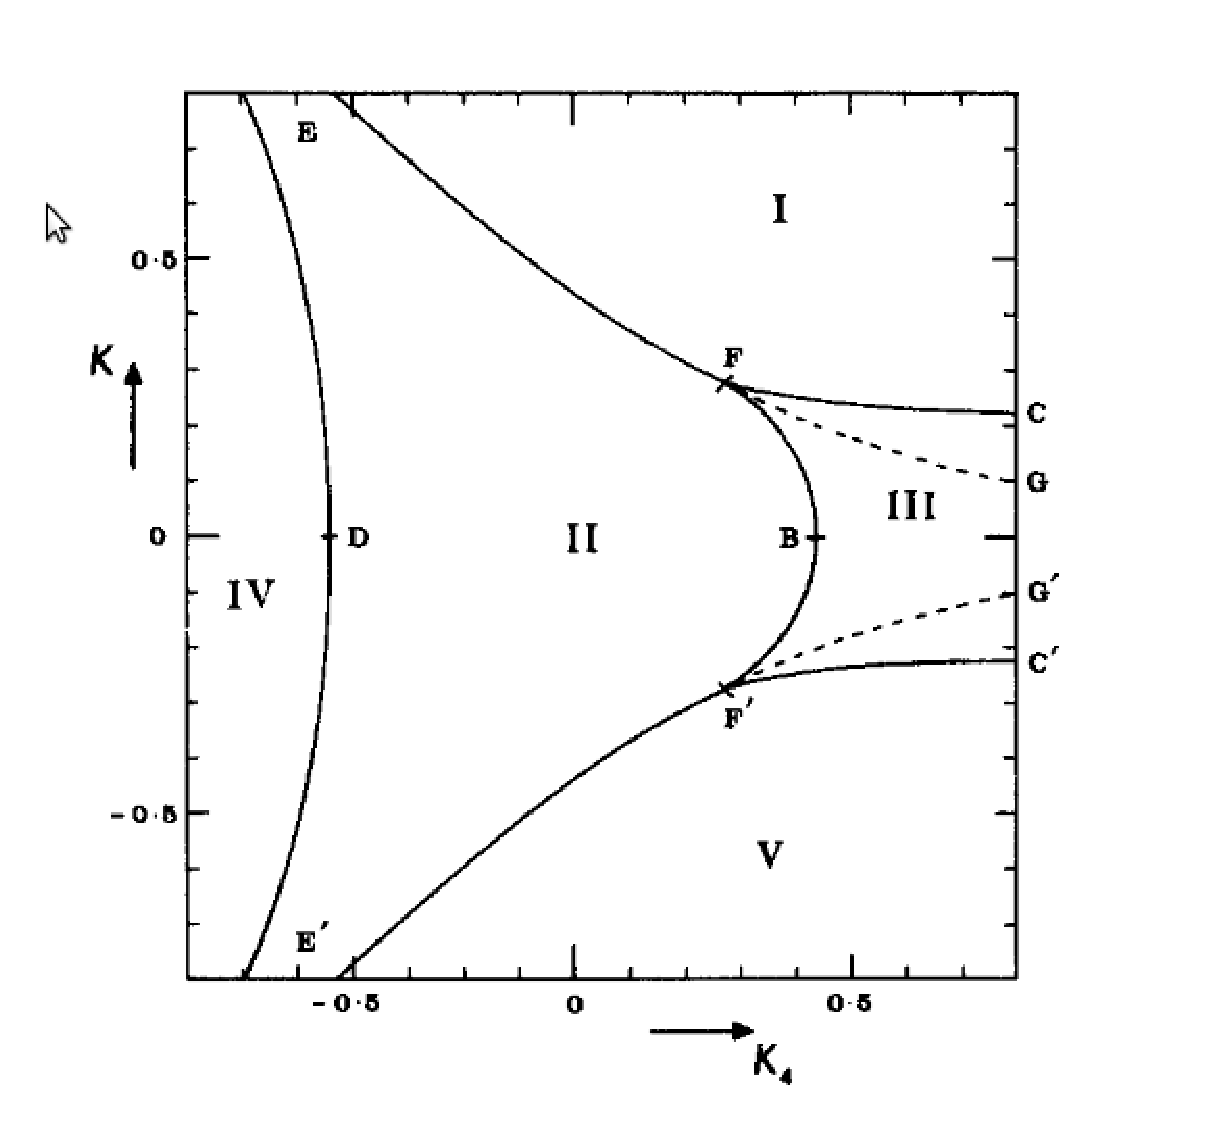
\includegraphics[scale=0.65]{graf/phases/AT_ph_diag_Baxter.eps}
\end{center}
\caption{Diagrama de fases del modelo Ashkin-Teller. El sistema se encuentra en diferentes estados de orden en cada una de las regiones I, II, III, IV y V.
 Se indican con letras (B, C, C$'$, D, E, E$'$, F, F$'$, G, G$'$) algunos puntos en los que $K_{4}$ y $K$ son conocidos exactamente.}
\label{fig:AT_ph_diag_Baxter}
\end{figure}

El diagrama de fases del modelo AT representado en la figura \ref{fig:AT_ph_diag_Baxter} en t\'erminos de $K=J/kT$ y $K_{4}=J_{4}/kT$,
 fue obtenido, utilizando resultados que surgieron de varios métodos (simulaciones MC, teoría de campo medio y grupo de renormalización),
 en 1980 por Ditzian et. al. \cite{AT_3D_phdiag}. En él se evidencian cinco regiones caracterizadas por diferentes estados de orden.\\
Además de los parámetros de orden usuales para un sistema magnético dados en la sección \ref{sec:teoria}, es útil definir unos que midan el grado de orden entre
ambos tipos de spines, gobernado por el acoplamiento $K_{4}$, para ello consideraremos el momento magnético dado por el producto $\sigma\tau$:

\begin{center} 
\begin{eqnarray}
	\label{eq:op_Mst}
	\mean{\sigma\tau}&=&\frac{1}{L^{2}}\sum_{ij}\sigma_{ij}\tau_{ij} \\
	\label{eq:op_stagMst}
	\mean{\sigma\tau}_{AF}&=&\frac{1}{L^{2}}\sum_{ij}(-1)^{(i+j)}\sigma_{ij}\tau_{ij}
\end{eqnarray}
\end{center}
 donde $ij$ representa los \'indices de un sitio en la red bidimensiional y las sumatorias se extienden sobre toda la red.
El parámetro de orden $\mean{\sigma \tau}$ es una medida de la proporci\'on de pares de spines $\sigma-\tau$ en los que $\sigma$ y $\tau$
 se encuentran alineados en el mismo sitio de red, toma su valor máximo solo cuando los spines en ambos planos se encuentran en el mismo estado de orden;
 $\mean{\sigma\tau}_{AF}$ mide el orden alternado de los pares $\sigma-\tau$,
 este par\'ametro puede ser no nulo incluso cuando $\mean{\sigma}$ y $\mean{\tau}$ son ambos nulos.\\

En la regi\'on I del diagrama de fases de la fig. \ref{fig:AT_ph_diag_Baxter} ambos acoplamientos, $K$ y $K_{4}$, son suficientemente fuertes, $\mean{\sigma}$ y $\mean{\tau}$ est\'an ordenandos de forma independiente
 ($\mean{\sigma}=\pm \mean{\tau}$) y $\mean{\sigma\tau}$ es no nulo, y por lo tanto,% esto ocurre cuando $K_{4}/K \gtrsim -1$ y
 el sistema presenta orden ferromagn\'etico total. En la regi\'on II, los acoplamientos son muy d\'ebiles y el sistema est\'a
 completamente desordenado ($\mean{\sigma}$, $\mean{\tau}$ y $\mean{\sigma\tau}$ son nulos).
La regi\'on III presenta orden parcial, $K_{4}$ supera a $K$ en toda la regi\'on, permitiendo que $\sigma\tau$ presente orden ferromagn\'etico mientras que $\tau$ y $\sigma$
 est\'an independientemente desordenados.
La regi\'on IV se da para valores grandes y negativos de $K_{4}$ los spines $\sigma$ y $\tau$ se encuentran desordenados, mientras que $\sigma\tau$ presenta orden de tipo anti-ferromagn\'etico.
La región V es similar a la I, pero $\sigma$ y $\tau$ están ordenados de manera anti-ferromagnética.\\

La curva E-F que delimita las regiones I y II en el diagrama de fases de la Fig. \ref{fig:AT_ph_diag_Baxter} resulta de particular interés, ya que
 sobre ella los exponentes críticos del modelo varian continuamente con el acoplamiento $K_{4}$. La expresión analítica que define dicha curva
 en términos de las constantes de acoplamiento del modelo AT \cite{AT_fan1972a,baxter_book} puede obtenerse a partir de un análisis de simetrías sobre el modelo 8V
 y está dada por:
\\ 
\begin{equation}
	\label{eq:lincrit}
	e^{(-2K_{4})}=\sinh{(2K)} , \; \; \; \; K_{4}<K,
\end{equation}
\\
 el punto E corresponde a $K_{4}/K =-1$, $K\rightarrow\infty$, donde $\mu=2\pi/3$, y el punto F a $K_{4}=K$, con $\mu=0$.\\
Si se analiza el caso $K_{4}=0$, se obtiene el punto crítico $K=K_{c}^{Ising}$ para el modelo de Ising, donde $K_{c}^{Ising}$ está dado por:
\\
\begin{equation}
	\label{eq:isingcrit}
	\sinh{(2K_{c}^{Ising})}=1, %\; \; \; \; K_{c}^{Ising}\eqsim 0.440686...
\end{equation}
\\
Respecto a las curvas que separan el resto de las fases en el diagrama de la fig. \ref{fig:AT_ph_diag_Baxter}, sólo la curva E$'$-F$'$,
 que se obtiene a partir de la línea E-F negando $K$, es conocida analíticamente, y sobre ella los exponentes críticos varian continuamente.
 Las prolongaciones F-G y F$'$-G$'$ (en líneas punteadas en la fig. \ref{fig:AT_ph_diag_Baxter}) no representan
 curvas críticas. Si bien las curvas F-B y F-C no son conocidas analíticamente, el punto B ha sido estimado como $K=0$, $K_{4}=K_{c}^{Ising}$ y el punto C es
 $K_{4}=\infty$, $K=\frac{1}{2}K_{c}^{Ising}$. De la misma forma, la curva E-D-E$'$ no es conocida anal\'iticamente, pero el punto D corresponde a $K=0$, $K_{4}=-K_{c}^{Ising}$.
 Los exponentes críticos sobre estas tres últimas curvas tienen valores fijos, y se espera que estos sean los del modelo de Ising bidimensional.\\


	\subsection{Resultados}
\label{sec:results_AT}
%\subsubsection{Verificación del modelo AT}

\begin{figure}[ht!]
\begin{center}
\includegraphics[scale=0.8]{graf/phases/multi_ising_sigma_tau_inkscape.eps}
\end{center}
\caption{En el caso $K_{4}=0$ el comportamiento de los spines $\sigma$ y los $\tau$ es el del modelo de Ising en una red cuadrada.
 (a): en las medidas de la magnetización del sistema ($|M_{\sigma}|=\mean{\sigma}$, $|M_{\tau}|=\mean{\tau}$) puede observarse la transici\'on de fase de segundo orden en $K_{c}^{Ising}$,
 (b): la susceptibilidad magn\'etica presenta un pico abrupto en $K_{c}^{Ising}$ que se vuelve m\'as pronunciado a medida que
 aumenta el tamaño del sistema, deber\'ia transformarse en una divergencia para $L\rightarrow \infty$.(c): A partir
 del cumulante de cuarto orden es posible determinar el punto cr\'itico para un sistema finito, (d): La ubicaci\'on del
 punto cr\'itico se obtiene de la intersecci\'on entre los cumulantes para diferentes valores de $L$.}
\label{fig:multi_ising_sigma_tau}
\end{figure}

Nuestro objetivo en esta sección es comprobar la fidelidad del algoritmo utilizado en las simulaciones con el modelo AT. Para ello estudiamos
 el comportamiento del sistema en diferentes situaciones en las que los resultados son conocidos, ya sea analíticamente o a partir de otros estudios numéricos.\\
Hemos tenido en cuenta primero la situación más sencilla, en la que el acoplamiento entre spines $\sigma$ y $\tau$, $K_{4}$, es nulo y el sistema puede separarse
 en dos modelos de Ising bidimensionales independientes. Luego abordamos el estudio del comportamiento del sistema en las diferentes fases descriptas en
 la sección \ref{sec:AT_model} y la determinación de las líneas críticas que se observan en el diagrama de la Fig. \ref{fig:AT_ph_diag_Baxter}. Por último antes de considerar
 el sistema con defectos, estudiamos el comportamiento no universal del exponente crítico de la magnetización en el modelo AT sobre la línea E-F del diagrama de fases.\\

%\begin{figure}[ht!]
%\begin{center}
%\includegraphics[scale=0.8]{graf/phases/multi_ising_sigma.eps}
%\end{center}
%\caption{En el caso $K_{4}=0$ el comportamiento de los spines $\sigma$ es el del modelo de Ising en una red cuadrada.
 %(a): en las medidas de la magnetización del sistema ($|M|=\mean{\sigma}$) puede observarse la transici\'on de fase de segundo orden en $K_{c}^{Ising}$,
 %(b): la susceptibilidad magn\'etica presenta un pico abrupto en $K_{c}^{Ising}$ que se vuelve m\'as pronunciado a medida que
 %aumenta el tamaño del sistema, deber\'ia transformarse en una divergencia para $L\rightarrow \infty$.(c): A partir
 %del cumulante de cuarto orden es posible determinar el punto cr\'itico para un sistema finito, (d): La ubicaci\'on del
 %punto cr\'itico se obtiene de la intersecci\'on entre los cumulantes para diferentes valores de $L$.}
%\label{fig:multi_ising_sigma}
%\end{figure}

Los datos analizados en esta sección surgen de medidas realizadas para los parámetros de orden $\mean{\alpha}$, $\mean{\alpha}_{AF}$,
 $\mean{\sigma\tau}$ y $\mean{\sigma\tau}_{AF}$ ($\alpha=\sigma, \tau$), definidos en las ecuaciones \ref{eq:op_Ms}, \ref{eq:op_stagMs}, \ref{eq:op_Mst} y
 \ref{eq:op_stagMst}, y sus momentos de orden 2 y 4, a partir de los que se pueden obtener el cumulante de cuarto orden y la
 susceptibilidad (ecs. \ref{eq:cumul4} y \ref{eq:suscept}) que permiten
 caracterizar la transición de fase y determinar el punto crítico.
Dado que nuestro objetivo en esta sección es reproducir las propiedades del modelo AT sin defectos, hemos optado por considerar sistemas de tamaños relativamente
 pequeños, $L=16,24,32$, a fines de reducir el tiempo de procesamiento en cada caso.
Para estos tamaños se realizaron corridas de hasta $3\times 10^{5}$ TMC, luego de un período de equilibrio de $3\times 10^{5}$ TMC, para los tamaños más grandes,
 y realizando promedios sobre 50 muestras independientes.\\

%\begin{figure}[ht!]
%\begin{center}
%\includegraphics[scale=0.8]{graf/phases/multi_ising_tau.eps}
%\end{center}
%\caption{Esta figura es similar a la figura \ref{fig:multi_ising_sigma}, pero se representan la magnetización ($|M|=\mean{\tau}$), susceptibilidad y cumulante de cuarto orden en función de $K$
 %para los spines $\tau$ en el caso $K_{4}=0$.}
%\label{fig:multi_ising_tau}
%\end{figure}

\subsubsection{Sistema desacoplado ($K_{4}=0$)}

Consideremos en primer lugar el caso en el cual $K_{4}=0$ que corresponde a dos modelos de Ising desacoplados, para los cuales
 se espera obtener una transición de fase de segundo orden para el valor $K = K_{c}^{Ising}$ determinado por la ec. (\ref{eq:isingcrit}).
 Para analizar esta transición hemos calculado la magnetización, la susceptibilidad magnética y el cumulante de cuarto orden
 como funciones de $K$ y para diferentes valores de $L$.\\
En la Fig. \ref{fig:multi_ising_sigma_tau} puede observarse el comportamiento de (a) los parámetros de orden $\abs{M_{\sigma,\tau}}$, (b) el cumulante de cuarto orden $U_{4}$ y
 (c) la susceptibilidad magnética asociada, característicos
 de una transición de fase de este tipo. A medida que aumenta el tamaño del sistema la transición en (a) se vuelve mas abrupta y el pico de la susceptibilidad en (c) tiende
 a una divergencia. Se observa además que el comportamiento es similar para los spines $\sigma$ y los $\tau$, ya que se trata, en este caso, de dos modelos de Ising independientes.\\
 
Hemos determinado el valor crítico de la constante de acoplamiento $K_{c}^{Ising}$ localizando las intersecciones de las gráficas de $U_{4}$
 para los spines $\sigma$ y $\tau$ para diferentes tamaños del sistema, $L=16,24,32$. Éstas pueden observarse en los gráficos $(d)$ en la figura \ref{fig:multi_ising_sigma_tau}.
% y \ref{fig:multi_ising_tau}.
 Los resultados obtenidos para los spines $\sigma$ y los $\tau$ están en buen acuerdo con el valor teórico de $K_{c}^{Ising}$ (ec. \ref{eq:isingcrit}):
 $K_{c}^{\sigma}=K_{c}^{\tau}=0.441(1)$.\\


\begin{figure}[h!]
	\begin{center}
		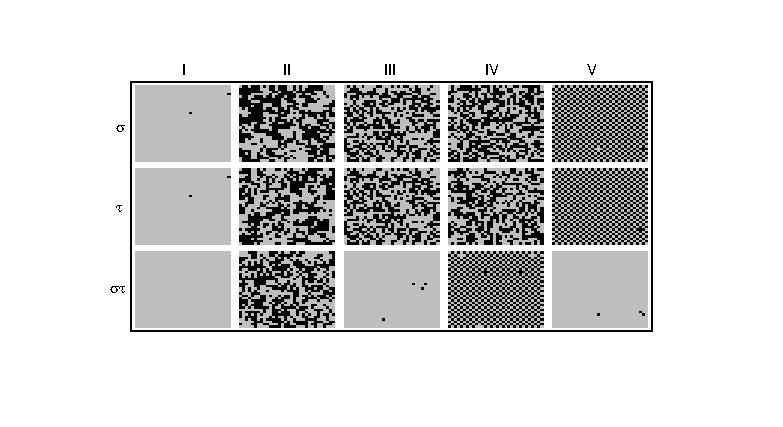
\includegraphics[scale=1]{graf/phases/multi_snaps32_horiz.eps}
	\end{center}
	\caption{Snapshots del sistema en las diferentes fases. Cada columna corresponde a una región diferente del diagrama de fases.
	En la fila superior se representan los spines $\sigma$, en la central los $\tau$ y en la inferior el producto $\sigma\tau$.
	Estos gráficos se han realizado para un sistema de tamaño $32\times 32$. Para la primera columna se ha tomado $K=0.5$ y $K_{4}=0.5$,
	es decir un estado del sistema correspondiente a la región I del diagramade fases. La segunda columna corresponde a la región II y se obtuvo con $K=0.2$ y $K_{4}=0$.
	La tercera columna se obtiene para $K=0.1$ y $K_{4}=0.75$ y pertenece la fase III. La cuarta columna }
	\label{fig:snaps_multi}
\end{figure} 

\subsubsection{Diagrama de fases para el caso acoplado $K_{4}\neq 0$}

Una vez analizado el caso desacoplado, pasamos a considerar un valor de $K_{4}$ no nulo, verificando las diferentes fases que presenta el modelo AT.
La figura \ref{fig:snaps_multi} muestra instantáneas del sistema en cada fase, imágenes que representan la red bidimensional en las que se utilizan diferentes tonalidades
 para indicar el estado de spin en que se encuentra cada sitio. Considerando solo dos tonalidades (claro y oscuro) el estado del modelo AT en un instante particular
 puede representarse por dos redes (spines $\sigma$ y $\tau$). En esta representación gráfica se hacen claras las diferentes fases asociadas a los valores de $K$ y $K_{4}$
 que se muestran en la Fig. \ref{fig:AT_ph_diag_Baxter}.
Cada columna corresponde a una de las regiones en el diagrama de fases, mientras que las filas, de arriba hacia abajo, corresponden a los estados de los spines
 $\sigma$, $\tau$ y del producto $\sigma\tau$. Estas medidas fueron realizadas para una red cuadrada de $32\times 32$.\\

En la primer columna se muestra la configuración para $K=0.5$ y $K_{4}=0.5$, que corresponde a la región I del diagrama de fases de
 la Fig. \ref{fig:AT_ph_diag_Baxter}, el sistema se encuentra completamente ordenado, todos los spines, tanto $\sigma$ como $\tau$, están en el mismo estado y
 por lo tanto también su producto.
En la columna 2 se presenta el caso $K=0.2$, $K_{4}=0$, en el que los spines $\sigma$ y los $\tau$ se encuentran desordenados de manera independiente,
 y por ello $\sigma\tau$ presenta también un estado sin orden alguno. Esto corresponde a la región II en la Fig. \ref{fig:AT_ph_diag_Baxter}.
En la columna 3 se observa como los spines $\sigma$ y $\tau$ pueden estar desordenados, mientras que su producto presenta un estado ordenado. Esta
 situación, correspondiente a la región III del diagrama de fases (Fig. \ref{fig:AT_ph_diag_Baxter}), es observada para un valor pequeño de las
 interacciones $\sigma-\sigma$ y $\tau-\tau$, $K=0.1$, y un acoplamiento relativamente fuerte para la interacción $\sigma-\tau$, $K_{4}=0.75$.
En cambio si el valor de $K_{4}$ es negativo, los spines $\sigma$ se acoplan a los $\tau$ de manera anti-ferromagnética, lo que puede verse en
 la columna 4 de la figura \ref{fig:snaps_multi} donde se ha elegido $K_{4}=-0.75$, en correspondencia con la región IV de la figura \ref{fig:AT_ph_diag_Baxter}.
Por último, en la columna 5, se ha considerado el caso en que $K$ es negativo, $K=-0.75$ y $K_{4}=0.1$, produciéndose un orden alternado para los $\sigma$ y los $\tau$,
 mientras que el producto $\sigma\tau$ permanece en un estado de orden ferromagnético. Este caso es representativo de la región V del diagrama de fases (Fig. \ref{fig:AT_ph_diag_Baxter}).\\

\begin{figure}[h!]
	\begin{center}
		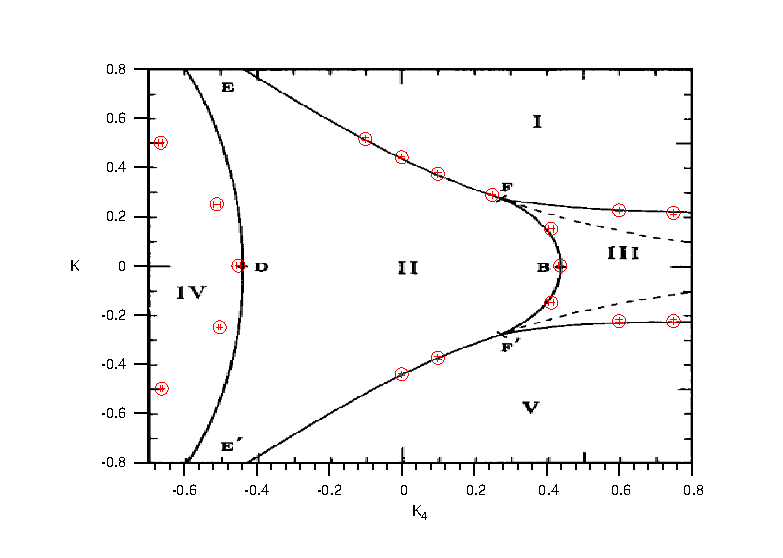
\includegraphics[scale=1]{graf/phases/new_phase_diag_back.eps}
	\end{center}
	\caption{Se presentan los puntos obtenidos en este trabajo para las transiciones de fase del modelo AT sobre el diagrama de fases publicado por Baxter\cite{baxter_book}.
	En el caso de la transici\'on II$\rightarrow$IV, la curva es solo representativa, no se ha determiando su expresi\'on anal\'itica.}
	\label{fig:phase_diag_back}
\end{figure}

\begin{figure}[h!]
	\begin{center}
		\includegraphics[scale=0.8]{graf/phases/multi_AT_I_II_c.eps}
	\end{center}
	\caption{En el caso $K_{4}=0.25$ la transición entre las fases I y II, localizada sobre la curva E-F, es similar a la que ocurre en el modelo de Ising.
	El valor crítico de $K$ es menor a $K_{c}^{Ising}$.(a): magnetización ($|M|=\mean{\sigma}$), puede observarse la transici\'on de fase de segundo orden en $K\simeq 0.287(1)$,
	(b): la susceptibilidad magn\'etica presenta un pico abrupto en $K_{c}^{Ising}$ que se vuelve m\'as pronunciado a medida que
	aumenta el tamaño del sistema, deber\'ia transformarse en una divergencia para $L\rightarrow \infty$.(c): A partir
	del cumulante de cuarto orden es posible determinar el punto cr\'itico para un sistema finito, (d): La ubicaci\'on del
	punto cr\'itico se obtiene de la intersecci\'on entre los cumulantes para diferentes valores de $L$.}
	\label{fig:multi_AT_I_II_c}
\end{figure}

\begin{figure}[h!]
	\begin{center}
		\includegraphics[scale=0.8]{graf/phases/new_multi_AT_II_IV_b.eps}
	\end{center}
	\caption{La transición entre las fases II y IV, localizada sobre la línea E-E'
	puede estudiarse mediante el parámetro de orden $\mean{\sigma\tau}_{AF}$, utilizando un valor fijo de $K=0.377$.
	El comportamiento de las magnitudes $\abs{M}_{\sigma\tau}^{AF}$, $\chi_{\sigma\tau}^{AF}$ y $U_{4\sigma\tau}^{AF}$
	corresponde al de una transici\'on de fase de segundo orden.}
	%\caption{La transición entre las fases II y III, localizada sobre la línea F-F' puede estudiarse mediante el parámetro de orden $\mean{\sigma\tau}_{AF}$.
	%El punto B se encuentra en $K=0$, $K_{4}=K_{c}^{Ising}$.(a): magnetización ($|M|=\mean{\sigma}$), puede observarse la transici\'on de fase de segundo orden en $K\simeq 0.287(1)$,
	%(b): la susceptibilidad magn\'etica presenta un pico abrupto en $K_{c}^{Ising}$ que se vuelve m\'as pronunciado a medida que
	%aumenta el tamaño del sistema, deber\'ia transformarse en una divergencia para $L\rightarrow \infty$.(c): A partir
	%del cumulante de cuarto orden es posible determinar el punto cr\'itico para un sistema finito, (d): La ubicaci\'on del
	%punto cr\'itico se obtiene de la intersecci\'on entre los cumulantes para diferentes valores de $L$.}
	\label{fig:multi_AT_II_IV_b}
\end{figure}

Mediante el mismo procedimiento que el utilizado en la transición de fase para $K_{4}=0$ % método del determinante de cuarto orden
 hemos determinado varios puntos ($K$, $K_{4}$) correspondientes a las curvas cr\'iticas del diagrama
 de la Fig. \ref{fig:AT_ph_diag_Baxter}. En la Fig. \ref{fig:phase_diag_back} se resumen
 dichos resultados numéricos superpuestos al diagrama de fases ya conocido, con el que se obtiene un excelente acuerdo,
 excepto en el caso de la curva E-D-E', en el que existe cierta diferencia. Este caso se discutirá más adelante.
%Las curvas cr\'iticas en el diagrama ($K$, $K_{4}$) para las transiciones entre las
 %fases enumeradas anteriormente han sido determinados de la misma forma que en
 %la transición para $K_{4}=0$, utilizando el método del cumulante de cuarto orden.
%Los resultados hallados para todas las transiciones de fase estudiadas concuerdan con el diagrama de fases de la Fig. \ref{fig:AT_ph_diag_Baxter},
 %y pueden verse superpuestos a este en la Fig. \ref{fig:phase_diag_back}, los c\'irculos rojos corresponden a los resultados n\'umericos obtenidos
 %en este trabajo.
Las figuras \ref{fig:multi_AT_I_II_c} y \ref{fig:multi_AT_II_IV_b} muestran el comportamiento
 de las magnitudes $\abs{M}$, $\chi$ y $U_{4}$ en las cercanías de los puntos críticos.
 La figura \ref{fig:multi_AT_I_II_c} corresponde al caso de
 la transición entre las fases I y II para un valor de $K_{4}$ diferente de $0$ donde se utiliz\'o
 $M_{\sigma}=\mean{\sigma}$ como par\'ametro de orden. Las curvas muestran el mismo comportamiento que en el caso
 $K_{4}=0$, pero puede verse que el valor crítico obtenido para $K$ es diferente.
 La figura \ref{fig:multi_AT_II_IV_b}
  corresponde a la transici\'on entre las fases II y IV, caraterizada por el parámetro de orden $\abs{M_{\sigma\tau}^{AF}}=\mean{\sigma\tau}_{AF}$,
  en los gr\'aficos (a-d) puede verse que el
  comportamiento del par\'ametro de orden $\mean{\sigma\tau}_{AF}$, la susceptibilidad $\chi_{\sigma\tau}^{AF}$
  y el cumulante de cuarto orden es el correspondiente a una transici\'on de fase de segundo orden.\\
 
\begin{figure}[h!]
	\begin{center}
		\includegraphics[scale=0.85]{graf/phases/phases_EF.eps}
	\end{center}
	\caption{Transiciones de fase sobre la línea E-F, definida por (\ref{eq:lincrit}), para diferentes valores de $K_{4}=-0.1, 0, 0.1, 0.25$. La curva con rayas
	corresponde al resultado analítico.}
	\label{fig:ph_EF}
\end{figure}
 
La forma de la curva que separa las fases I y II, incluyendo el caso $K_{4}=0$, (línea crítica E-F  de la Fig. \ref{fig:AT_ph_diag_Baxter}) es conocida con exactitud y
 está definida por la ec. (\ref{eq:lincrit}). A fines de reproducir este resultado teórico utilizando nuestra implementación del modelo AT hemos determinado el valor crítico de $K$ para diferentes
 valores de $K_{4}$ a partir de medidas de los parámetros de orden $\mean{\sigma}$ y $\mean{\tau}$ y sus momentos.
En la figura \ref{fig:ph_EF} puede observarse el acuerdo entre los resultados obtenidos para $K$ utilizando diferentes valores de $K_{4}$ y la representación gráfica de la
 ec. (\ref{eq:lincrit}) en el plano $K - K_{4}$.\\

En la transición entre las fases II y III el sistema pasa de una fase completamente desordenada a otra que exhibe orden parcial, los spines $\sigma$ y los $\tau$ se encuentran
 también desordenados, pero de forma tal que su producto presenta orden ferromagnético. Este orden puede detectarse a través del parámetro de orden $\mean{\sigma\tau}$,
 que describe una transición de segundo orden y presenta un comportamiento similar al de $\mean{\sigma}$ en los casos anteriores.
Aunque la forma exacta de línea crica F-F' que separa las fases II y III no se conoce analíticamente, se sabe que el punto identificado con la letra B
 corresponde a $K=0$, $K_{4}=K_{c}^{Ising}$. Nuestros resultados numéricos están en completo acuerdo con esto.\\

La fase IV está también parcialmente ordenada y se caracteriza por el orden alternado del producto $\sigma\tau$, por lo tanto midiendo el parámetro de orden $\mean{\sigma\tau}_{AF}$
 (dado en (\ref{eq:op_stagMst})) en función de $K_{4}$ y para diferentes valores de $K$ pueden determinarse algunos puntos correspondientes a la línea de la transición II$\rightarrow$IV.
 En la figura \ref{fig:AT_ph_diag_Baxter} la línea que separa las fases II y IV es sólo representativa, ya que el único punto que es conocido exactamente sobre esta línea es el punto D,
 que corresponde a $K=0$, $K_{4}=-K_{c}^{Ising}$. Hemos realizado medidas para determinar esta curva, tomando diferentes valores de $K$, obteniendo los puntos
 ($K=-0.5$, $K_{4}=-0.66..$), ($K=-0.25$, $K_{4}=-0.51..$), ($K=0.5$, $K_{4}=-0.665(5)$) y ($K=0.25$, $K_{4}=-0.51(5)$) que pueden observarse en la figura \ref{fig:phase_diag_back}.\\

En el caso de la transici\'on entre las fases II y IV, si bien el comportamiento de la l\'inea E-E' coincide con el correspondiente
 al diagrama de referencia, nuestros resultados sugieren que los valores de $K_{4}$ necesarios para que el sistema presente el orden de la fase IV
 deben ser mayores en magnitud.\\

Para valores negativos de $K$, los spines $\sigma$ tienden a alinearse antiferromagnéticamente entre sí, y si $K_{4}$ es suficientemente grande, se produce además un alineamiento 
ferromagnético para el producto $\sigma\tau$. Esto ocurre al atravesar la curva E'-F', que separa las regiones II y V en el diagrama de fases. Midiendo los parámetros de orden
 $\mean{\sigma}_{AF}$, $\mean{\tau}_{AF}$ y $\mean{\sigma\tau}$, obtuvimos algunos puntos sobre esta curva (Fig. \ref{fig:phase_diag_back}).\\

%~ \begin{figure}[h!]
	%~ \begin{center}
		%~ 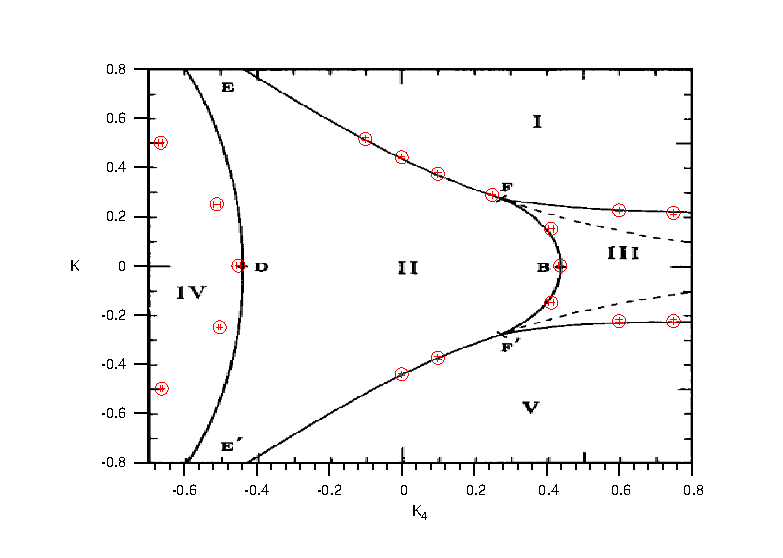
\includegraphics[scale=1]{graf/phases/new_phase_diag_back.eps}
	%~ \end{center}
	%~ \caption{Se presentan los puntos obtenidos en este trabajo para las transiciones de fase del modelo AT sobre el diagrama de fases publicado por Baxter\cite{baxter_book}.
	%~ En el caso de la transici\'on II$\rightarrow$IV, la curva es solo representativa, no se ha determiando su expresi\'on anal\'itica.}
	%~ \label{fig:phase_diag_back}
%~ \end{figure}

Los resultados hallados para todas las transiciones de fase estudiadas concuerdan con el diagrama de fases de la Fig. \ref{fig:AT_ph_diag_Baxter},
 y pueden verse superpuestos a este en la Fig. \ref{fig:phase_diag_back}, los c\'irculos rojos corresponden a los resultados n\'umericos obtenidos
 en este trabajo.\\
\newpage


\section{Modelo AT con un defecto en forma de línea.}
\label{sec:AT_line_intro}
En esta sección definiremos el defecto introducido al modelo AT y presentaremos los resultados que hemos obtenido sobre el mismo.\\

	\subsection{Introducción de un defecto en el modelo AT.}
\label{sec:AT_line}

%La introducción de defectos que rompen la invarianza traslacional en el plano genera un cambio en las propiedades físicas del sistema en la zona del defecto,
 %cuya extensión depende de la longitud de correlación $\xi$. En la región crítica, donde $\xi$ diverge, la influencia de las perturbaciones causadas
 %por el defecto en las magnitudes locales, como las funciones de correlación y la magnetización del defecto, ha sido analizada en términos de
 %la teoría de escala \cite{inhomog_sys}.\\
%Según la teoría de escala, cuando las longitudes en el sistema son re-escaleadas en un factor $b>1$, los parámetros que miden la desviación de ciertas magnitudes
 %respecto del punto crítico (por ejemplo la temperatura, $t=\abs{T-T_{c}}$) se modifican en un factor $b^{d-x}$, donde $d$ es la dimensión del sistema y $x$
 %la dimensión de escala de las cantidades conjugadas (por ejemplo la densidad de energía, en el caso de la temperatura). Cuando $d-x>0$ el parámetro es llamado
 %relevante y crece al producirse el cambio de escala; en cambio si $d-x<0$, su comportamiento es decreciente y es llamado irrelevante; finalmente, el parámetro es
 %considerado marginal si $d=x$. Mientras que los parámetros irrelevantes pueden hacerse desaparecer mediante transformaciones de escala, los relevantes y marginales
 %conducen a variaciones en el comportamiento crítico del sistema, estos últimos en particular producen exponentes variables.\\
%Cuando se introduce un defecto de dimensión $d^{*}$ en un sistema de dimensión $d$ el acoplamiento correspondiente al defecto se transforma según $b^{d^{*}-x}$ ante
 %un cambio de escala, donde $d^{*}$ es la dimensión del defecto y, utilizando algunos argumentos de la teoría de escala, se llega a $x=d-\frac{1}{\nu}$. De esta
 %forma la relevancia del defecto queda determinada por los valores de $d$, $d^{*}$ y $\nu$, es relevante si se cumple la condición $d-d^{*}<\frac{1}{\nu}$, y es marginal
 %en el caso $d-d^{*}=\frac{1}{\nu}$.\\
 
Un defecto en un sistema magnético puede ser representado mediante la modificación de las constantes de acoplamiento en una determinada región espacial del sistema.
Por ejemplo un borde, o una superficie libre, en un sistema bidimensional corresponde a modificar un número infinito de enlaces, este caso ha sido ampliamente estudiado
para el modelo de Ising revelando que las propiedades críticas del sistema se ven modificadas en una región cercana la superficie, cuyo tamaño es del orden de la
 longitud de correlación, y por lo tanto son descriptas por un conjunto de exponentes críticos diferentes a los del sistema homogéneo (bulk).\\
 
\begin{figure}[h!]
\begin{center}
\includegraphics[scale=0.65]{graf/line_defect_sigma_tau_5x5.eps}
\end{center}
\caption{Defecto asim\'etrico en forma de línea. Los símbolos $\sigma$ y $\tau$ representan los diferentes tipos de spines y los segmentos que los unen
las constantes de acoplamiento entre ellos. La constante de acoplamiento entre los spines $\sigma$ se modifica sobre una l\'inea, indicada en color y con
 segmentos dobles, mientras que la constante de acoplamiento entre los spines $\tau$ conserva su valor en toda la red.}
\label{fig:line_defect_sigma}
\end{figure}

En este trabajo estudiaremos el comportamiento crítico local sobre un defecto con forma de línea en el modelo AT.
Introducimos un defecto asimétrico \cite{AT_naon} en el sistema modificando solo la interacción entre los spines de tipo $\sigma$ sobre una línea
del plano que los contiene (fig. \ref{fig:line_defect_sigma}), el acoplamiento entre los spines que yacen sobre el defecto y sus
 vecinos en la dirección perpendicular a la línea no se modifica, y dado que se trata del modelo AT 
 isotrópico, su valor $J$ es el mismo que para la interacción entre los spines $\tau$.
Llamando $J_{l}$ a la intensidad del defecto y considerando su contribución
 al Hamiltoniano del modelo AT (ec. \ref{eq:ham_AT}) en el caso isotrópico se obtiene:
\\
\begin{equation}
	\label{eq:line_pot}
	H_{AT}=-J\sum_{<ij,km>}(\sigma_{ij}\sigma_{km}+\tau_{ij}\tau_{km})-J_{4}\sum_{<ij,km>}\sigma_{ij}\sigma_{km}\tau_{ij}\tau_{km}-J_{l}\sum_{<ij,km>}\delta_{il}\sigma_{ij}\delta_{kl}\sigma_{km}
\end{equation}
donde las deltas en el último término hacen que la suma sea solo sobre los spines que se encuentran sobre la línea de defectos (sitios de la red con el primer índice igual a $l$).
De esta forma para $J_{l}=0$ se recupera el modelo AT sin defectos. La interacción entre los spines $\sigma$ que yacen sobre el defecto está dada por los términos primero y cuarto
 de este Hamiltoniano y por lo tanto el acoplamiento efectivo entre estos resulta $J+J_{l}$. Si bien el acoplamiento entre los spines $\tau$ no se modifica, el defecto tendrá influencia
 sobre su comportamiento debido a la conexión entre los spines $\sigma$ y los $\tau$ gobernada por la constante $J_{4}$.\\

Si se considera $K_{4}=0$ se obtienen dos modelos de Ising sin acoplamiento entre sí, uno con un defecto en forma de línea y otro sin defectos. El comportamiento
 del exponente crítico de la magnetización sobre la línea de defectos es diferente en cada uno de ellos. En el modelo con spines $\tau$ conserva su valor
 $\beta=\frac{1}{8}$ (el correspondiente al modelo de Ising), mientras que para los $\sigma$ se espera una dependecia del exponente con la intensidad del defecto $K_{l}=J_{l}/kT$:

\begin{equation}
	\label{eq:exp_crit_e0}
	x_{m}^{\sigma} = \frac{2}{\pi^{2}}arctan^{2}(e^{-2K_{l}}) , \; \; \; \; x_{m}^{\tau}=1/8, \; \; \; \; K_{4}=0.
\end{equation}
Esta relación fue hallada por Bariev \cite{AT_bariev_line} a partir de la solución exacta del modelo de Ising bidimensional con un defecto en forma de línea.\\

En el caso $K_{4}\neq 0$, la influencia del defecto sobre el comportamiento de los spines $\tau$ es gobernada por $K_{4}$. El comportamiento del
 exponente crítico de la magnetización asociado a ambos tipos de spines es algo complejo en este caso ya que la interacción efectiva entre los spines en la
 región en que el defecto se encuentra localizado depende de la competencia entre los acoplamientos $K$, $K_{4}$ y $K_{l}$. A continuación nos proponemos estudiar este
 comportamiento.\\

%El modelo de Ising bidimensional con un defecto en forma de línea fue estudiado por Bariev \cite{AT_bariev_line}, quien dedujo que el comportamiento de la magnetización
% local en función de la intensidad del defecto y la distancia a la línea, corresponde a leyes de potencia. Dado que para este modelo $d=2$, $d^{*}=1$ y $\nu=1$, el defecto
% resulta marginal y se espera que los exponentes críticos dependan de la intensidad del defecto.\\
%Bariev obtuvo esta dependencia para el exponente crítico de la magnetización sobre el defecto:
%\\
%\begin{equation}
%	\label{eq:exp_crit_bariev}
%	\beta_{l} = \frac{2}{\pi^{2}}arctan^{2}(e^{-2(K-K')}),
%\end{equation}
%\\

%donde $K$ es el acoplamiento entre spines del modelo de Ising y $K'$ el acoplamiento modificado, presente solo sobre el defecto.\\


	\subsection{Resultados}
\label{sec:results_AT_line}
%\subsubsection{Modelo AT con defecto en forma de línea}

Nuestro objetivo principal en el estudio del sistema AT con defecto es el de determinar la dependencia
 del exponente crítico de la función de correlación spin-spin $x_{corr}$ con la intensidad del acoplamiento entre los spines
 $\sigma$ y $\tau$ $K_{4}$. Como hemos mencionado en la sec. \ref{sec:teoria_escala} este exponente está directamente relacionado
 con el exponente crítico de la magnetización local de la línea de defectos $x_{m}$. Aprovechando esta conexión junto al hecho de que
 la determinación de este último exponente es más sencilla que la de $x_{corr}$, hemos realizado medidas de la magnetización sobre el defecto
 y a partir de ellas determinado el comportamiento de $x_{m}$.\\

Presentamos a continuación los resultados numéricos obtenidos en el estudio de la dependencia de
 $x_{m}^{\alpha}$ con la intensidad del defecto sobre la l\'inea E-F del diagrama de fases (Fig. \ref{fig:AT_ph_diag_Baxter}) definida por la ec. \ref{eq:lincrit}.
Los puntos sobre la l\'inea E-F pueden clasificarse seg\'un el valor del par\'ametro $\epsilon=K_{4}/K$, que representa el acoplamiento
 entre los spines $\sigma$ y los $\tau$:
$\epsilon<0$, los spines $\tau$ tienden a alinearse antiferromagnéticamente con los $\sigma$; $\epsilon=0$, no hay acoplamiento
 entre los $\tau$ y los $\sigma$; $\epsilon>0$, el acoplamiento es del tipo ferromagnético.
Al extremo E de la l\'inea E-F le corresponde el valor $\epsilon = -1$ en el l\'imite $K\rightarrow \infty$ y al punto F el valor $\epsilon = 1$.
 Una vez elegido el valor del par\'ametro $\epsilon$
 para una medida, los valores de $K_{4}$ y $K$ se determinan a  partir de la ec. \ref{eq:lincrit} y la relaci\'on $\epsilon=K_{4}/K$.\\

Debido al tamaño finito del sistema, el valor del exponente cr\'itico depende de $L$, y debe determinarse a partir de medidas de la magnetización para distintos tamaños,
 seg\'un la relación:

\begin{equation}
	\label{eq:magvsL}
	m_{l}^{\alpha}(L)\sim L^{-x_{m}^{\alpha}}, \; \; \; \; \alpha=\sigma , \tau .
\end{equation}
Hemos realizado medidas considerando tamaños hasta $L=128$ en una red cuadrada con condiciones de contorno periódicas.\\

\begin{figure}[h!]
\begin{center}
\includegraphics[width=\figwidth]{graf/exp/mls_vs_L_e0.eps}
\end{center}
\caption{Logaritmo de la magnetización sobre el defecto $m_{l}^{\sigma}$ en función del logaritmo del tamaño del sistema para diferentes valores de $K_{l}$,
la pendiente de estas rectas representa el valor del exponente cr\'itico $x_{m}^{\sigma}$.}
\label{fig:mls_vs_L_e0}
\end{figure}

\subsubsection{Sistema desacoplado: $\epsilon=0$}

Como ya hemos mencionado, en este caso el sistema se divide en dos modelos de Ising idenpendientes. Uno con un defecto en forma de l\'inea
 (spines $\sigma$) y otro que carece de defectos (spines $\tau$) y, por lo tanto, debe comportarse como el modelo de Ising bidimensional.
El resultado analítico para los exponentes $x_{m}^{\sigma}$ y $x_{m}^{\tau}$ (ec. \ref{eq:exp_crit_e0}) est\'a dado por:

\begin{equation*}
	\label{eq:exp_crit_e0}
	x_{m}^{\sigma} = \frac{2}{\pi^{2}}\arctan^{2}(e^{-2K_{l}}) , \; \; \; \; x_{m}^{\tau}=1/8, \; \; \; \; K_{4}=0
\end{equation*}

Dado que $\epsilon=0$, los resultados de esta secci\'on corresponden a los valores cr\'iticos de $K_{4}=0$ y $K=K_{c}^{Ising}$.
 mientras que para la intensidad del defecto hemos considerado diferentes valores entre $K_{l}=-0.4$ y $K_{l}=0.44$.
 Las medidas de la magnetizaci\'on sobre el defecto
 de los spines $\sigma$ en función de $L$ para estos valores de $K_{l}$ se muestran en la figura \ref{fig:mls_vs_L_e0} en escala logar\'itmica,
 claramente el comportamiento de $m_{l}$ se ajusta a una ley de potencias y los valores del exponente cr\'itico corresponden a la pendiente
 de cada una de las rectas (en este caso la dependencia del exponente con L es despreciable) . Los valores num\'ericos de dicho exponente en funci\'on de la intensidad del defecto se presentan en la Fig.
 \ref{fig:fit_arctan_e0}, donce puede verse que est\'an en completo acuerdo con el resultado anal\'itico (ec. \ref{eq:exp_crit_e0}),
 gr\'afico en l\'inea punteada.\\
En el caso de los spines $\tau$, el exponente cr\'itico $x_{m}^{\tau}$ es el mismo para todos los valores de $K_{l}$, y su valor coincide con el resultado
 conocido para el modelo de Ising sin defecto $x_{m}^{\tau}=\frac{1}{8}$.\\  

\begin{figure}[h!]
\begin{center}
\includegraphics[width=\figwidth]{graf/exp/fit_arctan_e0.eps}
\end{center}
\caption{Exponente crítico de la magnetización del defecto para $\epsilon=0$, la línea punteada representa el resultado teórico (\ref{eq:exp_crit_e0}).}
\label{fig:fit_arctan_e0}
\end{figure}

\subsubsection{Acoplamiento positivo: $\epsilon>0$}

Cuando el acoplamiento entre los spines $\sigma$ y los $\tau$, $\epsilon$, es diferente de cero, la magnetización del defecto
 no se comporta exactamente como una ley de potencias, es decir que los exponentes $x_{m}^{\sigma}$ y $x_{m}^{\tau}$ dependen del
 tamaño del sistema $L$. Hemos realizado medidas de la magnetizaci\'on sobre el defecto $m_{l}$ a fines de determinar la dependencia del
 exponente cr\'itico con el par\'ametro $\epsilon$. Todas estas medidas corresponden a puntos sobre la curva cr\'itica E-F
 en el plano ($K$, $K_{4}$), de forma que para una dado valor de $\epsilon$, $K$ y $K_{4}$ deben satisfacer la ec. \ref{eq:lincrit}.
 En la Fig. \ref{fig:desv} se observa la magnetización del defecto en función de $L$ (en escala logar\'itmica) para los casos
 $\epsilon=0$ y $\epsilon=0.75$, en el segundo caso puede apreciarse claramente una desviación respecto al comportamiento de una ley de potencias.

\begin{figure}[h!]
\begin{center}
\includegraphics[width=\figwidth]{graf/exp/desv_e0.75_vs_e0.eps}
\end{center}
\caption{Gráfico del logaritmo de $m_{l}^{\sigma}$ vs. el logaritmo de $L$ para una intesidad del defecto $K_{l}=-0.35$ en
 los casos $\epsilon=0$ y $\epsilon=0.75$, puede apreciarse la desviación respecto de una ley de potencias cuando $\epsilon\neq 0$.}
\label{fig:desv}
\end{figure}
Se espera que para valores muy grandes de $L$ la magnetización recupere su comportamiento como ley de potencias en función
 de $L$, y por lo tanto el exponente crítico efectivo tienda al valor correspondiente a un sistema de tamaño infinito,
 $x_{m}(L)\rightarrow x_{m}(\infty)$. Sin embargo el tamaño de sistema m\'aximo que puede ser alcanzado, manteniendo un tiempo de c\'alculo
 aceptable est\'a limitado, principalmente por la eficiencia del algoritmo utilizado cerca de las regiones cr\'iticas.
 
%Una primera aproximaci\'on al valor efectivo del exponente puede obtenerse a partir de la magnetización para dos valores diferentes
% del tamaño del sistema, $L$ y $bL$, tomando el logaritmo de la ec. (\ref{eq:magvsL}) y resolviendo para $x_{m}$:
%\\
%\begin{equation}
%	\label{eq:exp_eff}
%	x_{m}^{\alpha}(L) = \frac{\ln{m_{l}^{\alpha}(bL)}-\ln{m_{l}^{\alpha}(bL)}}{\ln{b}}, \; \; \; \; \alpha=\sigma , \tau .
%\end{equation}
%\\
Hemos considerado tres valores positivos diferentes de $\epsilon$, para cada uno de ellos medimos la magnetizaci\'on sobre el
 defecto para diferentes intensidades del defecto $K_{l}$. La figura \ref{fig:ml_vs_L_all}
 muestra gr\'aficos del logaritmo de $m_{l}^{\alpha}$ en funci\'on del logaritmo de $L$, por lo tanto la pendiente de estas curvas
 representa el exponente crítico efectivo $x_{m}^{\alpha}(L)$, ya que tomando el logaritmo de la ec.(\ref{eq:magvsL}), que lo define, se obtiene:
 
\begin{equation}
	\label{eq:logmagvsL}
	\ln{(m_{l}^{\alpha}(L))} \sim -x_{m}^{\alpha}\Ln{(L)}, \; \; \; \; \alpha=\sigma , \tau .
\end{equation}
 
\begin{figure}[h!]
\begin{center}
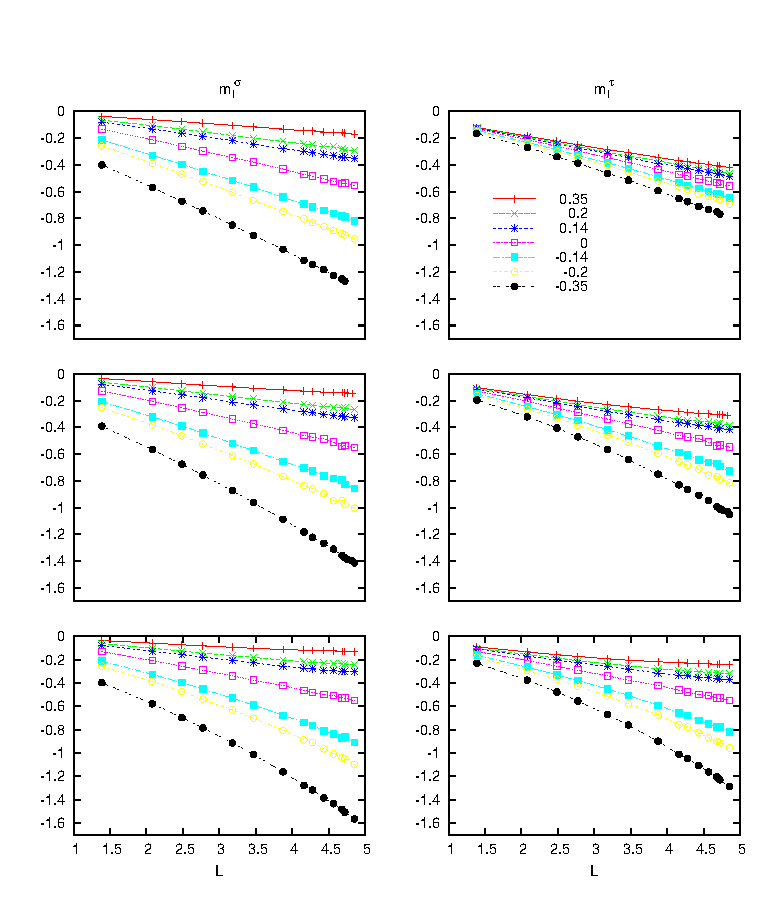
\includegraphics[width=\figwidth]{graf/exp/ml_vs_L_all.eps}
\end{center}
\caption{Gráfico del logaritmo de la magnetización sobre el defecto $m_{l}^{\alpha}$ en función del logaritmo del tamaño del
 sistema $L$. Cada fila corresponde a un valor diferente del acoplamiento entre los spines $\sigma$ y los $\tau$,
 $\epsilon=0.25, 0.5, 0.75$. En la columna de la izquierda se representan los datos para los spines $\sigma$ y en
 la columna derecha para los $\tau$. Cada uno de estos gr\'aficos contiene las medidas de $m_{l}^{\alpha}$ para cinco
 valores diferentes de la intensidad del defecto $K_{l}=-0.35, -0.2, -0.14, 0, 0.14, 0.2, 0.35$. La pendiente de las
 curvas disminuye para valores positivos de $K_{l}$ (s\'imbolos \textcolor{red}{$+$}, \textcolor{green}{$\times$}
 y \textcolor{blue}{$\times$}) y aumenta para los valores negativos de $K_{l}$ (\textcolor{cyan}{$\square$}, \textcolor{yellow}{$\circ$}
 y $\bullet$).}
\label{fig:ml_vs_L_all}
\end{figure}
Los resultados se presentan en un arreglo en el que la columna de la izquierda corresponde a los spines $\sigma$,
 la de la derecha a los $\tau$ y cada fila a un valor diferente de $\epsilon$ en orden creciente hacia abajo,
 $\epsilon=0.25,0.5,0.75$. Cada uno de los gr\'aficos contiene las curvas para cinco valores diferentes de $K_{l}$.
 Las tres curvas de menor pendiente en cada gr\'afico son para los valores  positivos de la intensidad del defecto
 (s\'imbolos \textcolor{red}{$+$}, \textcolor{green}{$\times$} y \textcolor{blue}{$*$}), en estos casos la
 pendiente disminuye a medida que aumenta el tamaño del sistema, por lo tanto el exponente
 $x_{m}^{\alpha}$ tiende a un valor $x_{m>}^{\alpha}$ menor al correspondiente al sistema libre de defectos, tanto para los espines
 $\tau$ como para los $\sigma$, y la desviación respecto del valor sin defectos aumenta a medida que el valor de $K_{l}$ se aparta de $0$.
 %Se espera que, para valores muy grandes de $L$, $x_{m>}^{\alpha}$ se aproxime a cero.
La curva central (\textcolor{magenta}{$\square$}) corresponde a $K_{l}=0$, tiene en todos los casos una pendiente muy pr\'oxima
 a $\frac{1}{8}$ y pr\'acticamente no muestra desviaciones de este valor al aumentar $L$.
Las tres curvas inferiores de cada gr\'afico, las de mayor pendiente, corresponden a valores negativos de la intensidad del defecto,
 en este caso el exponente crítico se aproxima a un valor $x_{m<}^{\alpha}$ mayor a $\frac{1}{8}$ y la desviación respecto al caso desacoplado
 es también más apreciable para los valores más negativos de $K_{l}$.\\

Los valores num\'ericos del exponente cr\'itico efectivo pueden obtenerse a partir de la magnetización para dos
 valores diferentes del tamaño del sistema, $L$ y $bL$, tomando el logaritmo de la ec. (\ref{eq:magvsL}) y resolviendo para $x_{m}$:
\begin{equation}
	\label{eq:exp_eff}
	x_{m}^{\alpha}(L) = \frac{\ln{m_{l}^{\alpha}(bL)}-\ln{m_{l}^{\alpha}(bL)}}{\ln{b}}, \; \; \; \; \alpha=\sigma , \tau .
\end{equation}

Si se grafican los valores obtenidos en funci\'on de la inversa del tamaño del sistema, $\frac{1}{L}$, el valor
del exponente en el l\'imite $L\rightarrow \infty$ puede estimarse determinando graficamente la intersecci\'on
de la extrapolaci\'on de la gr\'afica con la l\'inea vertical $L=0$. En nuestro caso, debido a la lenta convergencia
del algoritmo utilizado en la regi\'on cr\'itica, la extrapolaci\'on mencionada es muy dif\'icil de realizar. Por ejemplo, la Fig.\ref{fig:xfits}
muestra la gr\'afica obtenida de esta forma para $\epsilon=0.75$ y $K_{l}=-0.35$ donde se aprecian las fluctuaciones para L grande.
 Por ello hemos optado por determinar el
valor del exponente cr\'itico para el mayor valor del tamaño del sistema $L=128$ utilizado en las simulaciones ajustando un polinomio de orden $2$
a la gr\'afica de $\ln{(m_{l})}$ vs. $L$ (Fig. \ref{fig:xfits}-(a)), a partir del cual obtenemos el valor del exponente
evaluando la derivada en $L=128$. Mediante este procedimiento determinamos $x_{m}$ para todos los valores de $\epsilon$
y $K_{l}$ estudiados.
Su comportamiento se muestra en la Fig. \ref{fig:exps_st_all}
 para los tres valores de $\epsilon$ como funci\'on de $K_{l}$. Se incluyen
 tambi\'en con fines comparativos los datos para $\epsilon=0$ y el resultado te\'orico para ese mismo caso. La desviaci\'on
 respecto al caso desacoplado aumenta con la intensidad del acoplamiento $\epsilon$ y es mas fuerte para el exponente asociado
 a los spines $\sigma$ (s\'imbolos sin relleno en la figura, $\vartriangle$, $\circ$ y $\square$) que para el exponente $x_{m}^{\tau}$ asociado a los $\tau$
 (s\'imbolos $\blacktriangle$, $\bullet$ y $\blacksquare$).
Para valores positivos de $K_{l}$, $x_{m}^{\sigma,\tau}$ tiene un valor menor al que presenta para $K_{l}=0$, y se aproxima
 a cero a medida que $K_{l}$ aumenta.
Para valores negativos de $K_{l}$, los exponentes cr\'iticos son mayores que para el caso sin defecto y aumentan a medida que el
 valor absoluto de $K_{l}$ crece.\\
 
\begin{figure}[htbp!]
\begin{center}
\includegraphics[width=\figwidth]{graf/exp/mag_exp_e0.75_Jln0.35.eps}
\end{center}
\caption{(a) Magnetizaci\'on sobre el defecto en funci\'on de la inversa del tamaño del sistema, $\frac{1}{L}$ para
 $\epsilon=0.75$ y $K_{l}=-0.35$, la l\'inea punteada muestra el ajuste de un polinomio de grado $2$, (b) valor efectivo
  del exponente cr\'itico de la magnetizaci\'on obtenido utilizando la ec.(\ref{eq:exp_eff})
 para los puntos de la gr\'afica (a) tomados de a pares.}
\label{fig:xfits}
\end{figure}

\begin{figure}[h!]
\begin{center}
\includegraphics[width=\figwidth]{graf/exp/exp_all_01.eps}
\end{center}
\caption{Exponente crítico de la magnetización del defecto, en función de la intensidad $K_{l}$. Se muestran los resultados para $\epsilon=0.25,0.5,0.75$.
Los puntos del gráfico representados por símbolos sin relleno $\vartriangle$, $\circ$ y $\square$ corresponden a los spines $\sigma$, mientras que los 
representados por símbolos rellenos, $\blacktriangle$, $\bullet$ y $\blacksquare$, corresponden a los spines $\tau$. La línea horizontal punteada
indica el valor $\frac{1}{8}$, valor teórico del exponente para $K_{l}=0$.}
\label{fig:exps_st_all}
\end{figure}

El hecho de que el valor del exponente se aproxime a cero cuando la intensidad del defecto es grande y positiva, puede ser analizado
 en terminos de la transici\'on de fase orden-desorden para la l\'inea de defectos. Los spines que yacen sobre la l\'inea
 se encuentran acoplados entre s\'i por una constante efectiva $K_{ef}=K+K_{l}$ que es m\'as fuerte que su acoplamiento
 con los \'atomos que no est\'an sobre la l\'inea, es decir sus vecinos en la direcci\'on perpendicular a ésta. De esta forma,
 el defecto tiende a estar ordenado para valores de $K$ menores al valor cr\'itico para el plano, y se encuentra en ese estado cuando
 el resto del sistema transita del desorden al orden. Este comportamiento puede verse en la figura \ref{fig:line_enhdec3_e0.75}, donde
 se muestran los par\'ametros de orden $\mean{\sigma}$ y $\mean{\sigma}_{l}$ que miden el orden del plano formado por todos los spines
 de tipo $\sigma$ y de la l\'inea de defectos, respectivamente, en funci\'on del acoplamiento $K$, para una transici\'on de fase sobre
 la curva E-F.\\

\begin{figure}[h!]
\begin{center}
\includegraphics[width=\figwidth]{graf/exp/line_enhdec3_e0.75.eps}
\end{center}
\caption{Parámetros de orden $\mean{\sigma}$ (magnetizaci\'on del plano $\sigma$) y $\mean{\sigma}_{l}$ (magnetizaci\'on sobre el defecto)
 para una transici\'on de fase sobre la l\'inea E-F. Cuando la intensidad del defecto es positiva $K_{l}=0.35$, la l\'inea se ordena
 para valores de $K$ inferiores al valor cr\'tico para el plano. Es decir que se encuentra ordenada cuando ocurre la transici\'on para el plano.
 Cuando $K_{l}=-0.35$ la l\'inea est\'a desordenada durante la transici\'on de fase.}
\label{fig:line_enhdec3_e0.75}
\end{figure}

Siguiendo el mismo razonamiento para el caso en que la intensidad del defecto es negativa, el valor efectivo del acoplamiento entre \'atomos sobre
 el defecto es menor que el acoplamiento $K$ y en consecuencia la l\'inea de defectos se encuentra desordenada o en transici\'on al orden para el
 valor de $K$ que produce el ordenamiento del plano.\\

\subsubsection{Acoplamiento negativo: $\epsilon<0$}

Observando las gr\'aficas del logaritmo de la magnetizaci\'on en funci\'on del logaritmo de $L$ cuando $\epsilon$ es negativo (figura \ref{fig:ml_vs_L_neg_all})
 podemos ver que en este caso el comportamiento para los spines $\sigma$ es diferente que para los $\tau$.\\
Para los $\sigma$ ocurre
 lo mismo que en el caso $\epsilon>0$, la pendiente del logaritmo de la magnetizaci\'on para valores positivos del defecto
 es menor que para el caso libre de defecto, mientras que para un defecto con intesidad negativa la pendiente es mayor. Para los
 spines $\tau$, sin embargo el comportamiento es inverso, es decir, las pendientes son mayores cuando la intesidad del defecto
 es positiva y menores cuando es negativa.
La figura \ref{fig:exp_neg_e0.75}, muestra los exponentes cr\'iticos $x_{m}^{\sigma}$ y $x_{m}^{\tau}$, obtenidos mediante ajustes
 de segundo orden al igual que en el caso $\epsilon>0$, como funci\'on de la intensidad del defecto.\\


\begin{figure}[h!]
\begin{center}
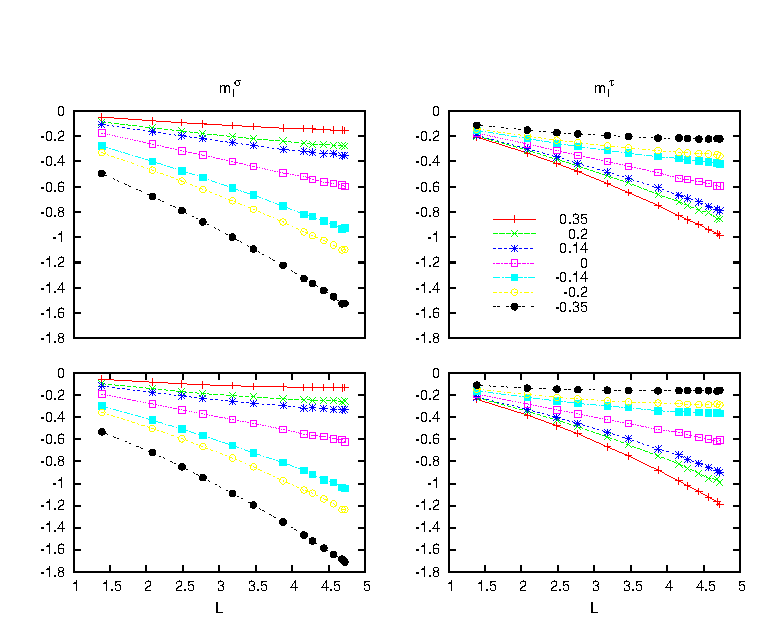
\includegraphics[width=\figwidth]{graf/exp/ml_vs_L_neg_all.eps}
\end{center}
\caption{Gráfico en escala logarítmica de la magnetización sobre el defecto $m_{l}^{\alpha}$ en función el tamaño del sistema $L$. Cada fila corresponde
 a un valor diferente del acoplamiento ($\epsilon=-0.5, -0.75$) entre los spines $\sigma$ y los $\tau$. En la columna de la izquierda se representan
 los datos para los spines $\sigma$ y en la columna derecha para los $\tau$.}
\label{fig:ml_vs_L_neg_all}
\end{figure}

\begin{figure}[h!]
\begin{center}
\includegraphics[width=\figwidth]{graf/exp/exp_all_neg_01.eps}
\end{center}
\caption{Exponente crítico de la magnetización del defecto, en función de la intensidad $K_{l}$ para $\epsilon <0$. Se muestran los resultados
 para $\epsilon=-0.5,-0.75$. Los puntos representados con símbolos sin relleno corresponden a los spines $\sigma$, su comportamiento es similar
 al hallado para valores positivos de $\epsilon$. El comportamiento del exponente asociado a los spines $\tau$ es contrario al hallado para
 $\epsilon>0$, estos valores están representados con símbolos rellenos.}
\label{fig:exp_neg_e0.75}
\end{figure}


\newpage

\section{Conclusiones}

En este trabajo hemos realizado un estudio del comportamiento crítico del modelo
 de Ashkin-Teller con un defecto en forma de línea utilizando el método de
 simulaciones computacionales Montecarlo.
 
Como punto de partida estudiamos las transiciones de fase en el modelo sin
 defectos y determinamos el diagrama de fases del sistema, obteniendo resultados
 en acuerdo con los encontrados en la literatura. Esta etapa sirvió también como
 verificación de nuestro algoritmo.

Respecto al modelo AT con un defecto en forma de línea constatamos la dependencia
 del exponente crítico asociado a la función de correlación spin-spin con la
 constante de acoplamiento del termino de interacción entre cuatro spines, ($K_{4}$).



%\input{apendices.tex}

% %  \bibliographystyle{plain}
%   \bibliographystyle{ieeetr}
%    \bibliography{biblio.bib}

% 

% \begin{thebibliography}{99}
% \input{planbiblio.tex}
% \end{thebibliography}
\bibliographystyle{plain}
\bibliography{phys.bib}

\end{document}
